\documentclass{article}
\usepackage{iclr2027_conference,times}
%%%%% NEW MATH DEFINITIONS %%%%%

\usepackage{amsmath,amsfonts,bm}

% Mark sections of captions for referring to divisions of figures
\newcommand{\figleft}{{\em (Left)}}
\newcommand{\figcenter}{{\em (Center)}}
\newcommand{\figright}{{\em (Right)}}
\newcommand{\figtop}{{\em (Top)}}
\newcommand{\figbottom}{{\em (Bottom)}}
\newcommand{\captiona}{{\em (a)}}
\newcommand{\captionb}{{\em (b)}}
\newcommand{\captionc}{{\em (c)}}
\newcommand{\captiond}{{\em (d)}}

% Highlight a newly defined term
\newcommand{\newterm}[1]{{\bf #1}}


% Figure reference, lower-case.
\def\figref#1{figure~\ref{#1}}
% Figure reference, capital. For start of sentence
\def\Figref#1{Figure~\ref{#1}}
\def\twofigref#1#2{figures \ref{#1} and \ref{#2}}
\def\quadfigref#1#2#3#4{figures \ref{#1}, \ref{#2}, \ref{#3} and \ref{#4}}
% Section reference, lower-case.
\def\secref#1{section~\ref{#1}}
% Section reference, capital.
\def\Secref#1{Section~\ref{#1}}
% Reference to two sections.
\def\twosecrefs#1#2{sections \ref{#1} and \ref{#2}}
% Reference to three sections.
\def\secrefs#1#2#3{sections \ref{#1}, \ref{#2} and \ref{#3}}
% Reference to an equation, lower-case.
\def\eqref#1{equation~\ref{#1}}
% Reference to an equation, upper case
\def\Eqref#1{Equation~\ref{#1}}
% A raw reference to an equation---avoid using if possible
\def\plaineqref#1{\ref{#1}}
% Reference to a chapter, lower-case.
\def\chapref#1{chapter~\ref{#1}}
% Reference to an equation, upper case.
\def\Chapref#1{Chapter~\ref{#1}}
% Reference to a range of chapters
\def\rangechapref#1#2{chapters\ref{#1}--\ref{#2}}
% Reference to an algorithm, lower-case.
\def\algref#1{algorithm~\ref{#1}}
% Reference to an algorithm, upper case.
\def\Algref#1{Algorithm~\ref{#1}}
\def\twoalgref#1#2{algorithms \ref{#1} and \ref{#2}}
\def\Twoalgref#1#2{Algorithms \ref{#1} and \ref{#2}}
% Reference to a part, lower case
\def\partref#1{part~\ref{#1}}
% Reference to a part, upper case
\def\Partref#1{Part~\ref{#1}}
\def\twopartref#1#2{parts \ref{#1} and \ref{#2}}

\def\ceil#1{\lceil #1 \rceil}
\def\floor#1{\lfloor #1 \rfloor}
\def\1{\bm{1}}
\newcommand{\train}{\mathcal{D}}
\newcommand{\valid}{\mathcal{D_{\mathrm{valid}}}}
\newcommand{\test}{\mathcal{D_{\mathrm{test}}}}

\def\eps{{\epsilon}}


% Random variables
\def\reta{{\textnormal{$\eta$}}}
\def\ra{{\textnormal{a}}}
\def\rb{{\textnormal{b}}}
\def\rc{{\textnormal{c}}}
\def\rd{{\textnormal{d}}}
\def\re{{\textnormal{e}}}
\def\rf{{\textnormal{f}}}
\def\rg{{\textnormal{g}}}
\def\rh{{\textnormal{h}}}
\def\ri{{\textnormal{i}}}
\def\rj{{\textnormal{j}}}
\def\rk{{\textnormal{k}}}
\def\rl{{\textnormal{l}}}
% rm is already a command, just don't name any random variables m
\def\rn{{\textnormal{n}}}
\def\ro{{\textnormal{o}}}
\def\rp{{\textnormal{p}}}
\def\rq{{\textnormal{q}}}
\def\rr{{\textnormal{r}}}
\def\rs{{\textnormal{s}}}
\def\rt{{\textnormal{t}}}
\def\ru{{\textnormal{u}}}
\def\rv{{\textnormal{v}}}
\def\rw{{\textnormal{w}}}
\def\rx{{\textnormal{x}}}
\def\ry{{\textnormal{y}}}
\def\rz{{\textnormal{z}}}

% Random vectors
\def\rvepsilon{{\mathbf{\epsilon}}}
\def\rvtheta{{\mathbf{\theta}}}
\def\rva{{\mathbf{a}}}
\def\rvb{{\mathbf{b}}}
\def\rvc{{\mathbf{c}}}
\def\rvd{{\mathbf{d}}}
\def\rve{{\mathbf{e}}}
\def\rvf{{\mathbf{f}}}
\def\rvg{{\mathbf{g}}}
\def\rvh{{\mathbf{h}}}
\def\rvu{{\mathbf{i}}}
\def\rvj{{\mathbf{j}}}
\def\rvk{{\mathbf{k}}}
\def\rvl{{\mathbf{l}}}
\def\rvm{{\mathbf{m}}}
\def\rvn{{\mathbf{n}}}
\def\rvo{{\mathbf{o}}}
\def\rvp{{\mathbf{p}}}
\def\rvq{{\mathbf{q}}}
\def\rvr{{\mathbf{r}}}
\def\rvs{{\mathbf{s}}}
\def\rvt{{\mathbf{t}}}
\def\rvu{{\mathbf{u}}}
\def\rvv{{\mathbf{v}}}
\def\rvw{{\mathbf{w}}}
\def\rvx{{\mathbf{x}}}
\def\rvy{{\mathbf{y}}}
\def\rvz{{\mathbf{z}}}

% Elements of random vectors
\def\erva{{\textnormal{a}}}
\def\ervb{{\textnormal{b}}}
\def\ervc{{\textnormal{c}}}
\def\ervd{{\textnormal{d}}}
\def\erve{{\textnormal{e}}}
\def\ervf{{\textnormal{f}}}
\def\ervg{{\textnormal{g}}}
\def\ervh{{\textnormal{h}}}
\def\ervi{{\textnormal{i}}}
\def\ervj{{\textnormal{j}}}
\def\ervk{{\textnormal{k}}}
\def\ervl{{\textnormal{l}}}
\def\ervm{{\textnormal{m}}}
\def\ervn{{\textnormal{n}}}
\def\ervo{{\textnormal{o}}}
\def\ervp{{\textnormal{p}}}
\def\ervq{{\textnormal{q}}}
\def\ervr{{\textnormal{r}}}
\def\ervs{{\textnormal{s}}}
\def\ervt{{\textnormal{t}}}
\def\ervu{{\textnormal{u}}}
\def\ervv{{\textnormal{v}}}
\def\ervw{{\textnormal{w}}}
\def\ervx{{\textnormal{x}}}
\def\ervy{{\textnormal{y}}}
\def\ervz{{\textnormal{z}}}

% Random matrices
\def\rmA{{\mathbf{A}}}
\def\rmB{{\mathbf{B}}}
\def\rmC{{\mathbf{C}}}
\def\rmD{{\mathbf{D}}}
\def\rmE{{\mathbf{E}}}
\def\rmF{{\mathbf{F}}}
\def\rmG{{\mathbf{G}}}
\def\rmH{{\mathbf{H}}}
\def\rmI{{\mathbf{I}}}
\def\rmJ{{\mathbf{J}}}
\def\rmK{{\mathbf{K}}}
\def\rmL{{\mathbf{L}}}
\def\rmM{{\mathbf{M}}}
\def\rmN{{\mathbf{N}}}
\def\rmO{{\mathbf{O}}}
\def\rmP{{\mathbf{P}}}
\def\rmQ{{\mathbf{Q}}}
\def\rmR{{\mathbf{R}}}
\def\rmS{{\mathbf{S}}}
\def\rmT{{\mathbf{T}}}
\def\rmU{{\mathbf{U}}}
\def\rmV{{\mathbf{V}}}
\def\rmW{{\mathbf{W}}}
\def\rmX{{\mathbf{X}}}
\def\rmY{{\mathbf{Y}}}
\def\rmZ{{\mathbf{Z}}}

% Elements of random matrices
\def\ermA{{\textnormal{A}}}
\def\ermB{{\textnormal{B}}}
\def\ermC{{\textnormal{C}}}
\def\ermD{{\textnormal{D}}}
\def\ermE{{\textnormal{E}}}
\def\ermF{{\textnormal{F}}}
\def\ermG{{\textnormal{G}}}
\def\ermH{{\textnormal{H}}}
\def\ermI{{\textnormal{I}}}
\def\ermJ{{\textnormal{J}}}
\def\ermK{{\textnormal{K}}}
\def\ermL{{\textnormal{L}}}
\def\ermM{{\textnormal{M}}}
\def\ermN{{\textnormal{N}}}
\def\ermO{{\textnormal{O}}}
\def\ermP{{\textnormal{P}}}
\def\ermQ{{\textnormal{Q}}}
\def\ermR{{\textnormal{R}}}
\def\ermS{{\textnormal{S}}}
\def\ermT{{\textnormal{T}}}
\def\ermU{{\textnormal{U}}}
\def\ermV{{\textnormal{V}}}
\def\ermW{{\textnormal{W}}}
\def\ermX{{\textnormal{X}}}
\def\ermY{{\textnormal{Y}}}
\def\ermZ{{\textnormal{Z}}}

% Vectors
\def\vzero{{\bm{0}}}
\def\vone{{\bm{1}}}
\def\vmu{{\bm{\mu}}}
\def\vtheta{{\bm{\theta}}}
\def\va{{\bm{a}}}
\def\vb{{\bm{b}}}
\def\vc{{\bm{c}}}
\def\vd{{\bm{d}}}
\def\ve{{\bm{e}}}
\def\vf{{\bm{f}}}
\def\vg{{\bm{g}}}
\def\vh{{\bm{h}}}
\def\vi{{\bm{i}}}
\def\vj{{\bm{j}}}
\def\vk{{\bm{k}}}
\def\vl{{\bm{l}}}
\def\vm{{\bm{m}}}
\def\vn{{\bm{n}}}
\def\vo{{\bm{o}}}
\def\vp{{\bm{p}}}
\def\vq{{\bm{q}}}
\def\vr{{\bm{r}}}
\def\vs{{\bm{s}}}
\def\vt{{\bm{t}}}
\def\vu{{\bm{u}}}
\def\vv{{\bm{v}}}
\def\vw{{\bm{w}}}
\def\vx{{\bm{x}}}
\def\vy{{\bm{y}}}
\def\vz{{\bm{z}}}

% Elements of vectors
\def\evalpha{{\alpha}}
\def\evbeta{{\beta}}
\def\evepsilon{{\epsilon}}
\def\evlambda{{\lambda}}
\def\evomega{{\omega}}
\def\evmu{{\mu}}
\def\evpsi{{\psi}}
\def\evsigma{{\sigma}}
\def\evtheta{{\theta}}
\def\eva{{a}}
\def\evb{{b}}
\def\evc{{c}}
\def\evd{{d}}
\def\eve{{e}}
\def\evf{{f}}
\def\evg{{g}}
\def\evh{{h}}
\def\evi{{i}}
\def\evj{{j}}
\def\evk{{k}}
\def\evl{{l}}
\def\evm{{m}}
\def\evn{{n}}
\def\evo{{o}}
\def\evp{{p}}
\def\evq{{q}}
\def\evr{{r}}
\def\evs{{s}}
\def\evt{{t}}
\def\evu{{u}}
\def\evv{{v}}
\def\evw{{w}}
\def\evx{{x}}
\def\evy{{y}}
\def\evz{{z}}

% Matrix
\def\mA{{\bm{A}}}
\def\mB{{\bm{B}}}
\def\mC{{\bm{C}}}
\def\mD{{\bm{D}}}
\def\mE{{\bm{E}}}
\def\mF{{\bm{F}}}
\def\mG{{\bm{G}}}
\def\mH{{\bm{H}}}
\def\mI{{\bm{I}}}
\def\mJ{{\bm{J}}}
\def\mK{{\bm{K}}}
\def\mL{{\bm{L}}}
\def\mM{{\bm{M}}}
\def\mN{{\bm{N}}}
\def\mO{{\bm{O}}}
\def\mP{{\bm{P}}}
\def\mQ{{\bm{Q}}}
\def\mR{{\bm{R}}}
\def\mS{{\bm{S}}}
\def\mT{{\bm{T}}}
\def\mU{{\bm{U}}}
\def\mV{{\bm{V}}}
\def\mW{{\bm{W}}}
\def\mX{{\bm{X}}}
\def\mY{{\bm{Y}}}
\def\mZ{{\bm{Z}}}
\def\mBeta{{\bm{\beta}}}
\def\mPhi{{\bm{\Phi}}}
\def\mLambda{{\bm{\Lambda}}}
\def\mSigma{{\bm{\Sigma}}}

% Tensor
\DeclareMathAlphabet{\mathsfit}{\encodingdefault}{\sfdefault}{m}{sl}
\SetMathAlphabet{\mathsfit}{bold}{\encodingdefault}{\sfdefault}{bx}{n}
\newcommand{\tens}[1]{\bm{\mathsfit{#1}}}
\def\tA{{\tens{A}}}
\def\tB{{\tens{B}}}
\def\tC{{\tens{C}}}
\def\tD{{\tens{D}}}
\def\tE{{\tens{E}}}
\def\tF{{\tens{F}}}
\def\tG{{\tens{G}}}
\def\tH{{\tens{H}}}
\def\tI{{\tens{I}}}
\def\tJ{{\tens{J}}}
\def\tK{{\tens{K}}}
\def\tL{{\tens{L}}}
\def\tM{{\tens{M}}}
\def\tN{{\tens{N}}}
\def\tO{{\tens{O}}}
\def\tP{{\tens{P}}}
\def\tQ{{\tens{Q}}}
\def\tR{{\tens{R}}}
\def\tS{{\tens{S}}}
\def\tT{{\tens{T}}}
\def\tU{{\tens{U}}}
\def\tV{{\tens{V}}}
\def\tW{{\tens{W}}}
\def\tX{{\tens{X}}}
\def\tY{{\tens{Y}}}
\def\tZ{{\tens{Z}}}


% Graph
\def\gA{{\mathcal{A}}}
\def\gB{{\mathcal{B}}}
\def\gC{{\mathcal{C}}}
\def\gD{{\mathcal{D}}}
\def\gE{{\mathcal{E}}}
\def\gF{{\mathcal{F}}}
\def\gG{{\mathcal{G}}}
\def\gH{{\mathcal{H}}}
\def\gI{{\mathcal{I}}}
\def\gJ{{\mathcal{J}}}
\def\gK{{\mathcal{K}}}
\def\gL{{\mathcal{L}}}
\def\gM{{\mathcal{M}}}
\def\gN{{\mathcal{N}}}
\def\gO{{\mathcal{O}}}
\def\gP{{\mathcal{P}}}
\def\gQ{{\mathcal{Q}}}
\def\gR{{\mathcal{R}}}
\def\gS{{\mathcal{S}}}
\def\gT{{\mathcal{T}}}
\def\gU{{\mathcal{U}}}
\def\gV{{\mathcal{V}}}
\def\gW{{\mathcal{W}}}
\def\gX{{\mathcal{X}}}
\def\gY{{\mathcal{Y}}}
\def\gZ{{\mathcal{Z}}}

% Sets
\def\sA{{\mathbb{A}}}
\def\sB{{\mathbb{B}}}
\def\sC{{\mathbb{C}}}
\def\sD{{\mathbb{D}}}
% Don't use a set called E, because this would be the same as our symbol
% for expectation.
\def\sF{{\mathbb{F}}}
\def\sG{{\mathbb{G}}}
\def\sH{{\mathbb{H}}}
\def\sI{{\mathbb{I}}}
\def\sJ{{\mathbb{J}}}
\def\sK{{\mathbb{K}}}
\def\sL{{\mathbb{L}}}
\def\sM{{\mathbb{M}}}
\def\sN{{\mathbb{N}}}
\def\sO{{\mathbb{O}}}
\def\sP{{\mathbb{P}}}
\def\sQ{{\mathbb{Q}}}
\def\sR{{\mathbb{R}}}
\def\sS{{\mathbb{S}}}
\def\sT{{\mathbb{T}}}
\def\sU{{\mathbb{U}}}
\def\sV{{\mathbb{V}}}
\def\sW{{\mathbb{W}}}
\def\sX{{\mathbb{X}}}
\def\sY{{\mathbb{Y}}}
\def\sZ{{\mathbb{Z}}}

% Entries of a matrix
\def\emLambda{{\Lambda}}
\def\emA{{A}}
\def\emB{{B}}
\def\emC{{C}}
\def\emD{{D}}
\def\emE{{E}}
\def\emF{{F}}
\def\emG{{G}}
\def\emH{{H}}
\def\emI{{I}}
\def\emJ{{J}}
\def\emK{{K}}
\def\emL{{L}}
\def\emM{{M}}
\def\emN{{N}}
\def\emO{{O}}
\def\emP{{P}}
\def\emQ{{Q}}
\def\emR{{R}}
\def\emS{{S}}
\def\emT{{T}}
\def\emU{{U}}
\def\emV{{V}}
\def\emW{{W}}
\def\emX{{X}}
\def\emY{{Y}}
\def\emZ{{Z}}
\def\emSigma{{\Sigma}}

% entries of a tensor
% Same font as tensor, without \bm wrapper
\newcommand{\etens}[1]{\mathsfit{#1}}
\def\etLambda{{\etens{\Lambda}}}
\def\etA{{\etens{A}}}
\def\etB{{\etens{B}}}
\def\etC{{\etens{C}}}
\def\etD{{\etens{D}}}
\def\etE{{\etens{E}}}
\def\etF{{\etens{F}}}
\def\etG{{\etens{G}}}
\def\etH{{\etens{H}}}
\def\etI{{\etens{I}}}
\def\etJ{{\etens{J}}}
\def\etK{{\etens{K}}}
\def\etL{{\etens{L}}}
\def\etM{{\etens{M}}}
\def\etN{{\etens{N}}}
\def\etO{{\etens{O}}}
\def\etP{{\etens{P}}}
\def\etQ{{\etens{Q}}}
\def\etR{{\etens{R}}}
\def\etS{{\etens{S}}}
\def\etT{{\etens{T}}}
\def\etU{{\etens{U}}}
\def\etV{{\etens{V}}}
\def\etW{{\etens{W}}}
\def\etX{{\etens{X}}}
\def\etY{{\etens{Y}}}
\def\etZ{{\etens{Z}}}

% The true underlying data generating distribution
\newcommand{\pdata}{p_{\rm{data}}}
% The empirical distribution defined by the training set
\newcommand{\ptrain}{\hat{p}_{\rm{data}}}
\newcommand{\Ptrain}{\hat{P}_{\rm{data}}}
% The model distribution
\newcommand{\pmodel}{p_{\rm{model}}}
\newcommand{\Pmodel}{P_{\rm{model}}}
\newcommand{\ptildemodel}{\tilde{p}_{\rm{model}}}
% Stochastic autoencoder distributions
\newcommand{\pencode}{p_{\rm{encoder}}}
\newcommand{\pdecode}{p_{\rm{decoder}}}
\newcommand{\precons}{p_{\rm{reconstruct}}}

\newcommand{\laplace}{\mathrm{Laplace}} % Laplace distribution

\newcommand{\E}{\mathbb{E}}
\newcommand{\Ls}{\mathcal{L}}
\newcommand{\R}{\mathbb{R}}
\newcommand{\emp}{\tilde{p}}
\newcommand{\lr}{\alpha}
\newcommand{\reg}{\lambda}
\newcommand{\rect}{\mathrm{rectifier}}
\newcommand{\softmax}{\mathrm{softmax}}
\newcommand{\sigmoid}{\sigma}
\newcommand{\softplus}{\zeta}
\newcommand{\KL}{D_{\mathrm{KL}}}
\newcommand{\Var}{\mathrm{Var}}
\newcommand{\standarderror}{\mathrm{SE}}
\newcommand{\Cov}{\mathrm{Cov}}
% Wolfram Mathworld says $L^2$ is for function spaces and $\ell^2$ is for vectors
% But then they seem to use $L^2$ for vectors throughout the site, and so does
% wikipedia.
\newcommand{\normlzero}{L^0}
\newcommand{\normlone}{L^1}
\newcommand{\normltwo}{L^2}
\newcommand{\normlp}{L^p}
\newcommand{\normmax}{L^\infty}

\newcommand{\parents}{Pa} % See usage in notation.tex. Chosen to match Daphne's book.

\DeclareMathOperator*{\argmax}{arg\,max}
\DeclareMathOperator*{\argmin}{arg\,min}

\DeclareMathOperator{\sign}{sign}
\DeclareMathOperator{\Tr}{Tr}
\let\ab\allowbreak

\usepackage{hyperref}
\usepackage{url}
\usepackage{booktabs}
\usepackage{amsmath,amssymb,amsthm}
\usepackage{graphicx}
\usepackage{xcolor}
\usepackage{multirow}
\usepackage{caption}

\usepackage{placeins}
\newtheorem{proposition}{Proposition}
\newtheorem{lemma}{Lemma}
\newtheorem{corollary}{Corollary}
\newtheorem{remark}{Remark}
\newcommand{\ident}{\mathrm{ident}}
\newcommand{\invert}{\mathrm{invert}}
\newcommand{\recover}{\mathrm{recover}}
\newcommand{\pihalf}{$\pi_{0.5}$}
\newcommand{\ph}{\textsuperscript{\dag}}
\raggedbottom

\title{Distinguishing Repairable Deployment\\ Failures from Vision-Language-Action\\ Failures Before Rollout}

\author{Anonymous authors\\ Paper under double-blind review}

\begin{document}
\maketitle

\begin{abstract}
Vision-language-action policies that work in the lab often fail when the camera is bumped or the arm starts somewhere
new. We show that most of these failures are not the policy's fault, and that a robot can tell which ones it can fix
before running the policy at all. The robot uses its own body as a measuring instrument. Its encoders say where its arm
should appear in the image, and comparing that with where it does appear reveals how the camera moved. From this the
robot re-renders the view the policy was trained on, predicts how much of that view it can restore, and checks whether
its own measurement can be trusted. On LIBERO-Plus with three policy families, the correction repairs 61 of 100 camera
failures while breaking 18 of 140 successes ($p = 1.3\times10^{-6}$), resetting to the training start repairs all 47
starting-pose failures on untuned suites, and on a held-out policy a pre-registered test of the correction with a
refined pose passes (15 repaired, 3 broken, $p = 0.004$). Before any rollout, the fraction of the training view the
correction restores ranks which failures it will fix, even within a single perturbation category where benchmark labels
carry no information, and the calibration's own residual flags every failed measurement on the held-out policies.
Tracing each remaining failure to its cause, at most 8 of 100 camera failures of the development policy belong to the
policy, and the rest are failed measurements or views the camera can no longer see. We prove a minimax floor on
calibration from the body alone. All experiments are in simulation. With learned masks, calibration reaches about a
centimetre, but the closed-loop gain over the raw policy is not yet significant, and on real images mask quality
limits calibration.
\end{abstract}

\section{Introduction}

Vision-language-action (VLA) policies are evaluated under one condition and deployed under another. LIBERO-Plus
\citep{liberoplus} made the gap concrete. Moving the camera or the robot's initial pose takes policies that solve a
task nine times in ten down to fewer than three in ten. The usual response is to make the policy more robust, or to
wrap it by restoring the corrupted input stream \citep{rightstream,crt,byovla}, re-rendering the view
\citep{anycamvla,vistabot,gsvla}, or predicting the camera inside the policy \citep{fixedtofree}.

We ask a question that comes before any of these. A deployment shift is either a \emph{nuisance}, which changes how the
scene is observed but leaves the task alone and could in principle be inverted, or it changes the task itself.
Benchmarks label perturbations by category, and wrappers route their corrections by that label. The label does not say
what is fixable, though. A camera that orbits 20 degrees can be recovered and one turned 35 degrees away cannot, yet
both count as ``camera'' (Fig.~\ref{fig:teaser}). What decides the matter is whether the robot can \emph{measure} the
change and whether undoing it \emph{restores} what the policy was trained on, and both can be estimated before the
policy acts.

\textbf{The body as the instrument.} A robot carries one calibrated object everywhere it goes, namely itself. Its
encoders give its pose, and a kinematic model with a renderer gives where its silhouette must appear for any camera
pose. We use this to \emph{measure} the nuisance, to estimate how much of the training view undoing it would restore,
and to \emph{undo} it for a frozen policy. A deployable variant of the score takes every camera input from the robot's
own measurement (Sec.~\ref{sec:score}). Most closed-loop results use the simulator's segmentation and depth in place of
a robot segmenter and an RGB-D sensor, and Sec.~\ref{sec:ladder} replaces both with learned sensing.

\textbf{Contributions.}
(1) \emph{Diagnosis: most camera failures are not the policy's.} An interventional ladder attributes 17 of 100
OpenVLA-OFT (OFT) camera failures to failed measurement and 21 to lost views, and at most 8 to the policy
(Fig.~\ref{fig:glance}b, Sec.~\ref{sec:ladder}). Robustness numbers under camera shift therefore largely measure the observation path.
(2) \emph{Method: a correction from self-measurement with two pre-rollout signals.} The correction repairs 61 of 100
camera failures while breaking 18 of 140 successes ($p = 1.3\times10^{-6}$), resetting to the training start repairs
all 47 starting-pose failures on untuned suites, and on a held-out policy a pre-registered test passes (15 repaired, 3
broken, $p = 0.004$). Coverage predicts which failures a fix will repair. Within one perturbation category, where category-level predictors score 0.5, the score reaches 0.737 pooled held-out (coverage alone 0.684), replicated in a pre-registered test. The calibration residual says whether the measurement worked, and it flags all 44 held-out
failed calibrations (Sec.~\ref{sec:score},~\ref{sec:undo}).
(3) \emph{Theory: a minimax floor on body-only calibration.} Every estimator that sees only the robot's body, learned
or not, has worst-case pose error at least $1/(4\sigma_{\min})$ in the local regime, within $4\sqrt{d_\eta}$ of the
least-squares rate (Sec.~\ref{sec:theory}). This explains when body-only measurement can work at all.

\begin{figure}[t]
\centering
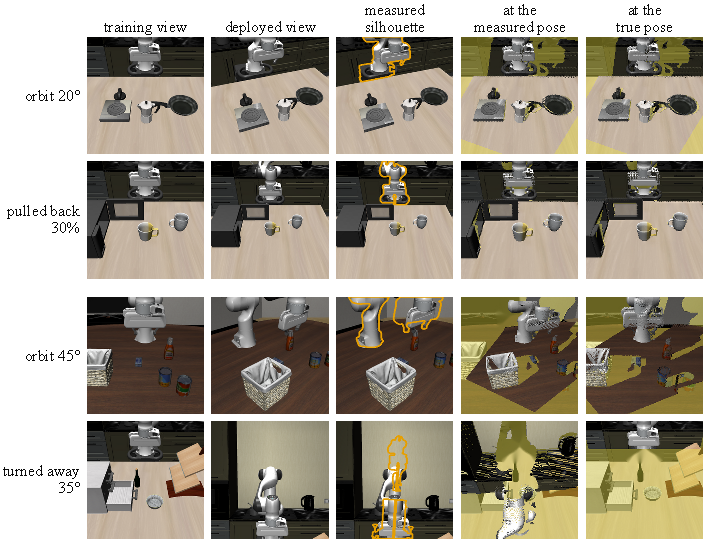
\includegraphics[width=0.86\linewidth]{figs/teaser.pdf}
\caption{Four deployed cameras (OFT tasks; policy-free renders). Columns: training view, deployed view, the silhouette
the robot fits its camera to from three probe poses (orange), the frame re-rendered into the training camera at the
measured pose (yellow: training-view pixels the deployed camera cannot see, giving the coverage), and at the true
pose. Rows 1-2
(recoverable; orbit 20 degrees, pulled back 30\%): measured within 0.1 and 1.1 cm, coverage 0.77 and 0.98. Row 3 (not
identified; orbit 45 degrees): the measurement fails (24.7 cm; the outline misses the arm), so the coverage it reports
(0.53) is not the view; at the true pose coverage is 0.64 and the view returns. Row 4 (not invertible; turned away 35
degrees): the measurement also fails (98 cm), self-measured coverage reads 0.48, and even the true pose covers 0.23 of
the training view.}
\label{fig:teaser}
\end{figure}

\begin{figure}[t]
\centering
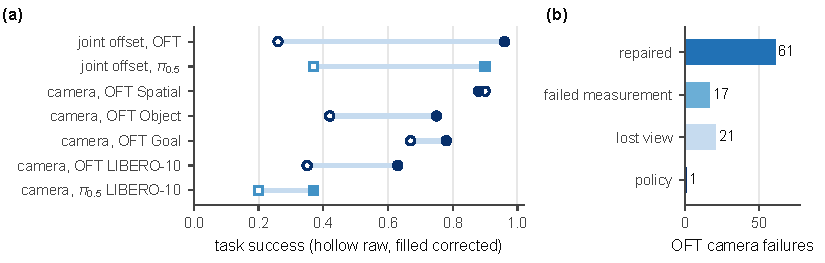
\includegraphics[width=\linewidth]{figs/glance.pdf}
\caption{Results at a glance. (a) Task success before (hollow) and after (filled) the correction on the same tasks and
seeds (Table~\ref{tab:suites}); on OFT the camera correction repairs 61 of 100 failures and breaks 18 of 140 successes,
most of them on Object and Goal; on Spatial, where raw success is already 0.90, it is neutral. (b) Where the 100 OFT camera failures go on the attribution ladder (Sec.~\ref{sec:ladder}). The
policy accounts for 1 of them, and for at most 8 at joint one-sided level 90\%.}
\label{fig:glance}
\end{figure}

\section{Related work}
\label{sec:related}
\textbf{Wrappers around frozen VLAs.} The closest work is Restoring the Right Stream \citep{rightstream}, a training-free
restoration on the same benchmark that routes each fix by input stream. BYOVLA \citep{byovla} edits task-irrelevant
image regions, CRT \citep{crt} restores corrupted inputs, and ProbeAct \citep{probeact} repairs actions. Right Stream
finds that robot-initial-state perturbations shift the proprioceptive stream, where image-space interventions have
limited leverage, which agrees with what our reset shows. None of these methods changes the viewpoint
geometry. CoRe \citep{core}, concurrent with this work, keeps a VLA frozen and realigns the robot and scene toward an
imagined continuation of a recent viable state. We differ from all of them in predicting, before any rollout, which
failures a correction can repair, and our baselines route by category and by the exact benchmark condition
(Sec.~\ref{sec:score}).
\textbf{Viewpoint.} AnyCamVLA \citep{anycamvla} re-renders the test view for a frozen VLA with learned view
synthesis from calibrated camera parameters; its depth-reprojection ablation is closest to our correction. We take
the pose from the robot's body and predict repairability. At the true pose our reprojection repairs 78 of 100 camera
failures, against 61 (Sec.~\ref{sec:ladder}). VistaBot \citep{vistabot} and GS-VLA \citep{gsvla} also synthesize the view, CamVLA \citep{fixedtofree} regresses the camera inside a retrained policy,
and \citet{spatialvla} trace viewpoint failures to spatial rather than physical modelling. Cross-view action consistency
\citep{crossview} fine-tunes a flow policy on LIBERO-Plus camera shifts. These methods retrain or adapt the policy, and
learned synthesis can hallucinate regions that a rigid z-buffered reprojection leaves as holes (filled from a stored
training view here). We keep the policy frozen and do not claim reprojection as ours.
\textbf{Robot as calibration target.} Render-and-compare robot pose estimation \citep{dream,robopose,ctrnet,gisr} and
mask-based hand-eye calibration \citep{easyhec,easyhecpp} are established, DROID \citep{droid} has been calibrated
offline from robot masks \citep{caliball,poseddroid}, and the conditioning of calibration Jacobians is a classical
observability measure \citep{bornmenq,nahvi}. Our silhouette calibration belongs to the EasyHeC and CtRNet family, so the
correction is built from known parts. What we add is the diagnosis it makes possible, and the use of the observability
measure at deployment to say when the robot's own measurement, and hence a small residual, can be trusted.
\textbf{Predicting failure.} RoboART \citep{roboart} predicts degradation under visual shift from the policy's own
embedding, and runtime monitors \citep{sentinel,faildetect,safevla,fiper,actprobe,triinfo} read the actions a policy
emits. VLA-Scope \citep{vlascope} and activation probes \citep{earlywarning}, both concurrent, predict failure from a
rollout of the policy, but neither asks whether a correction would repair it. Task-relevant shift \citep{farid},
identifiability for test-time adaptation \citep{ttaident}, selective adaptation \citep{selectivetta} and learned
canonicalisation \citep{kaba} are conceptual ancestors, and \citet{butterfly} and \citet{vincent} inform our
statistics. We predict \emph{repairability}, and we do it without the policy.

\section{Measure, predict, undo, check}
\label{sec:method}
Let $o = g(s;\eta)$ be the observation of state $s$ under nuisance parameters $\eta$ (camera pose, initial joint
configuration, illumination, sensor noise), let $\eta_0$ be the training setup, and let $\pi$ be a frozen policy. We
call a nuisance \emph{invertible} at $\eta$ if a map $T_\eta$, computed from the robot's own measurements, gives
$T_\eta(g(s;\eta)) \approx g(s;\eta_0)$ on the states the task visits. Fig.~\ref{fig:teaser} shows the loop, and
Appendix~\ref{app:defs} defines every quantity below by an explicit equation.

\textbf{Measure.} The robot records self-observations $z$ that need no knowledge of the scene. These are its joint
readings, the silhouette of its arm at a few end-effector poses it visits on purpose, the colour statistics of its own
links, and the noise level of its own pixels. The camera pose $\hat\eta_c$ minimises a silhouette chamfer plus a size
term over the visited poses, found by a coarse orbit grid, cross-entropy refinement and depth ICP, and it is accepted
only if it beats the training pose by a fixed factor (Eq.~\ref{eq:calloss}). Light and noise are measured as an affine
colour fit and a noise floor on the robot's own pixels.

\textbf{Predict.} The score and its first factor are (Eq.~\ref{eq:ident})
\begin{equation}
\recover(\eta) = \ident(\eta) \times \invert(\eta) \in [0,1], \qquad
\ident(\eta) = \min\Big(1, \frac{\sigma_{\min}(J_\phi(\eta))}{\sigma_{\min}(J_\phi(\eta_0))}\Big),
\label{eq:score}
\end{equation}
where $J_\phi$ is the finite-difference Jacobian of $z$ with respect to the condition's own parameter block, with
columns in fixed steps (1 cm and $1^\circ$ for the camera), and $\eta_0$ is the same base task unperturbed. The factor
asks whether the body still responds to the nuisance as it did in the training setup. In the registered score
$\ident$ is computed from the simulator at the true nuisance, which makes it policy-free but not self-measured. The
\emph{deployable score}\ph{} instead evaluates the camera Jacobian at the self-measured pose $\hat\eta_c$ and multiplies
by $\mathbb{1}[\rho \le \tau]$, where $\rho$ is the calibration's own final silhouette residual. By
Prop.~\ref{prop:r3oracle} the two versions of $\ident$ agree only where the calibration succeeded, and $\rho$ tells the
robot where that was. The second factor $\invert$ is self-measured and defined per channel. For a camera it is the
fraction of the $256^2$ training view that the reprojection from $\hat\eta_c$ fills on the first frame after the
measurement, which we call \emph{coverage} $c$. For light it is a split-half affine-invariant shading statistic of the
robot's links, and for noise the share of the added noise that the denoiser removes on the robot's pixels. It is 1 for
joint offsets and 0 for scene content, which has no inversion (App.~\ref{app:defs}). In use the two factors answer
two different questions. Coverage predicts which failures a fix will repair, and $\ident$ with the calibration residual says
whether the measurement behind it can be trusted. Every constant was frozen and
logged before the first episode of either held-out family.

\textbf{Undo.} A joint offset is undone by servoing to the training pose. A camera shift is undone by reprojecting into
the training camera with $\hat\eta_c$ and depth, z-buffered, with holes filled from a stored training-view reference.
Light is inverted through the affine fit unless the shading statistic says the change is not affine, and noise is
removed at the measured level. No weights change, and this \emph{evaluated wrapper} produces every headline number.
\textbf{Check (logged only).} A self-check warps the robot's observed silhouette with the same pose and depth and
compares it with where its kinematics place it in the training view (F1). The evaluated wrapper logs this but does not
act on it.

\subsection{What can be proved}
\label{sec:theory}
Near a pose $\eta$ the stacked self-observation over the probe poses $q_1, \dots, q_K$ is linear in the nuisance,
\begin{equation}
z = z_0 + J\delta + \epsilon, \qquad \epsilon \sim \mathcal N(0, \Sigma), \qquad \tilde J = \Sigma^{-1/2} J,
\label{eq:linmodel}
\end{equation}
with $\delta \in \mathbb{R}^{d_\eta}$ ($d_\eta = 6$ for a camera). The covariance $\Sigma$ carries spatially correlated
mask and depth errors, and i.i.d.\ pixel noise is the special case $\Sigma = \sigma^2 I$. Appendix~\ref{app:proofs}
proves each statement below under its stated conditions. They motivate the design, saying when body-only
measurement can work and why a small residual means something; the ranking itself is measured (Sec.~\ref{sec:score}).

\begin{proposition}[identifiability sets the rate]
\label{thm:rate}
Least squares on (\ref{eq:linmodel}) satisfies $\mathbb{E}\|\hat\delta - \delta\|^2 \le d_\eta/\sigma_{\min}(\tilde J)^2$,
and every estimator $\hat\delta(z)$, learned or not, satisfies
\begin{equation}
\inf_{\hat\delta}\ \sup_{\delta}\ \mathbb{E}_\delta\|\hat\delta(z) - \delta\| \ \ge\ \frac{1}{4\,\sigma_{\min}(\tilde J)}.
\label{eq:rate}
\end{equation}
Adding a probe pose never lowers $\sigma_{\min}(\tilde J)$.
\end{proposition}
The upper bound is the trace of the least-squares covariance $(\tilde J^\top \tilde J)^{-1}$, whose largest term is
$\sigma_{\min}(\tilde J)^{-2}$. The lower bound is Le Cam's two-point argument along the weakest singular direction $v$.
The hypotheses $\delta = 0$ and $\delta = tv$ are at Kullback-Leibler divergence $\tfrac12 t^2\sigma_{\min}(\tilde J)^2$,
so by Pinsker no test separates them better than $1 - t\sigma_{\min}(\tilde J)/2$, and $t = 1/\sigma_{\min}(\tilde J)$
gives (\ref{eq:rate}) (Props.~\ref{prop:r2cr},~\ref{prop:minimax}). Body-only calibration therefore has minimax error
$\Theta(1/\sigma_{\min}(\tilde J))$ within $4\sqrt{d_\eta}$, so $\sigma_{\min}$ sets how precisely the body can measure the nuisance, which is why a small calibration residual means something. The predicted log-log slope of error against $\sigma_{\min}$ is $-1$ and we measure $-0.84$
[$-1.60$, $-0.08$]. On 70 further camera units the error floor is consistent with a $1/\sigma_{\min}$ law (App.~\ref{app:facts}).

\begin{proposition}[a small residual bounds the pose error]
\label{thm:cert}
Let $J(\cdot)$ be $L$-Lipschitz in operator norm, $r$ the calibration residual and $\varepsilon$ the sensing error. If
$\|\hat\eta - \eta\| \le \sigma_{\min}(J(\eta))/L$, then
\begin{equation}
\|\hat\eta - \eta\| \le \frac{2\,(\|r\| + \|\varepsilon\|)}{\sigma_{\min}(J(\eta))}, \qquad
\big|\ident(\hat\eta) - \ident(\eta)\big| \le \frac{L\,\|\hat\eta - \eta\|}{\sigma_{\min}(J(\eta_0))}.
\label{eq:certmain}
\end{equation}
\end{proposition}
The first bound is Taylor's theorem with remainder at most $\tfrac L2\|\hat\eta - \eta\|^2$, which the basin condition
absorbs into half of $\sigma_{\min}\|\hat\eta - \eta\|$. The second is Weyl's inequality for singular values
(Props.~\ref{prop:cert},~\ref{prop:r3oracle}). This motivates the residual gate but does not certify it, since the gate thresholds the chamfer loss of
Eq.~\ref{eq:calloss} rather than $\|r\|$, and $L$ is not logged. Empirically the logged residual separates failed
calibrations at AUROC 1.000 on 89 camera units, and on the 40 units calibrated
within 2 cm $\ident$ at the measured pose differs from $\ident$ at the true pose by a median of 0.000.

\begin{proposition}[coverage is the invertible share]
\label{thm:cov}
Let $c$ be the fraction of the training view that the reprojection fills. The corrected frame's mean error is exactly
$(1-c)\,e_{\mathrm{hole}} + c\,e_V$, and any restoration from the deployed frame and stored side information has
error at least $(1-c)\,\bar e^\star$, with $\bar e^\star$ the Bayes risk on the unfilled pixels.
\end{proposition}
The identity splits the pixel sum over the filled set and its complement, and on an unfilled pixel no function of the deployed frame and the side information
does better than the conditional Bayes risk (Prop.~\ref{prop:cov}, Remark~\ref{prop:r3cov}). How coverage turns into repair is measured, not proved.

\begin{remark}[a motion-free test]
\label{thm:static}
If sensing and encoder errors are bounded, so that the rest-pose silhouette residual at the training camera satisfies
$r(q;\eta_0) \le \nu_{\max}$, then $r(q) > \nu_{\max}$ implies $\eta \ne \eta_0$.
\end{remark}
With an estimated floor this is a test with error rates bounded in Prop.~\ref{prop:switch} (used in Sec.~\ref{sec:cost}).


\section{Experiments}
\textbf{Setup.} LIBERO-Plus \citep{liberoplus}, four suites. Policies: OFT \citep{oft} with its per-suite checkpoints
(development family), and two held-out families on which no constant was chosen: \pihalf{} \citep{pi05} and OpenVLA
\citep{openvla} fine-tuned on LIBERO-10 (its released checkpoint and action statistics), a weaker policy (raw success
under shift: 0.19 over 210 LIBERO-Plus tasks; OFT 0.76; \pihalf{} 0.60 on 120 of them). A \emph{unit} is one
(condition, base task, seed), run raw and wrapped; it is \emph{repaired} if raw fails and wrapped succeeds,
\emph{broken} if the reverse, so $\mathrm{SR}_w - \mathrm{SR}_{\mathrm{raw}} = (R - B)/N$ over $N$ units. For prediction
a unit is (base task, condition), kept if the policy solves the base task unperturbed and its perturbed raw episode
fails (App.~\ref{app:defs}). The \emph{category label} is whether a wrapper routing by LIBERO-Plus category would apply
a correction (binary); the \emph{category rate} is the repair rate of the unit's category fit on OFT. The \emph{frame}
is the observation handed to the policy. The \emph{graded sweep} applies 24 conditions (nominal; 7 camera, 6 light, 4
noise, 3 joint, 3 background) to 10 base tasks. Set A is the first 30 LIBERO-10 camera tasks and set B the next 30.
Simulator segmentation and depth stand in for an RGB-D sensor and a robot segmenter (Sec.~\ref{sec:ladder}).
\textbf{Statistics.} AUROC is the Mann-Whitney statistic with ties counted one half, positive class ``repaired'';
intervals are percentile bootstraps over units (2{,}000 resamples, seed 0) and, in brackets, over base tasks. Paired
comparisons use the exact two-sided McNemar test on discordant units (Eq.~\ref{eq:mcnemar}). The one primary
pass/fail test is the pooled OFT camera McNemar. The score AUROC on the two held-out families was registered as a
descriptive quantity, with no pass criterion. The rest are secondary, with Holm-adjusted $p$ in Table~\ref{tab:holm}. Analyses designed after the main results are marked \ph; tests registered
before their data existed are listed with their outcomes in Appendix~\ref{app:prereg}.

\subsection{The recoverability score}
\label{sec:score}


\begin{figure}[t]
\centering
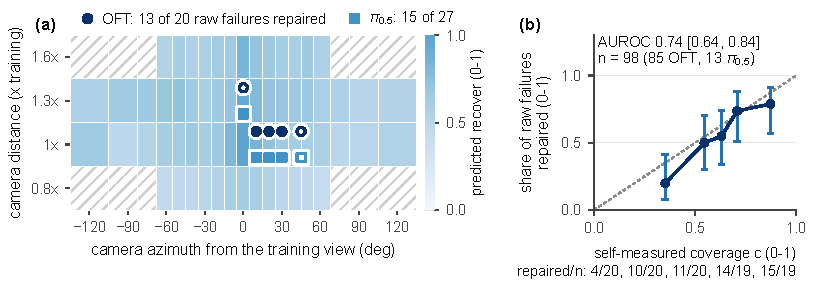
\includegraphics[width=\linewidth]{figs/envelope.pdf}
\caption{(a) The policy-free score $\recover$ over 88 camera placements $\times$ 3 base tasks (264 renders; mean over
the three base tasks; blue ramp; hatched: not rendered) with the graded sweep's outcomes at its five standard camera
placements (orbit 10, 20, 30, 45 degrees, pull-back 1.3; look-aways in Fig.~\ref{fig:tilt}), on base tasks each policy
solves unperturbed (OFT circles in the upper third of a cell, \pihalf{} squares in the lower third; filled: at least
half of the raw failures at that placement repaired; OFT 13 of 20 raw failures repaired, \pihalf{} 15 of 27).
$\ident \ge 0.9$ on 199 of the 264 task-placements, so $\recover$ tracks coverage. (b) Every LIBERO-Plus camera task
that logged coverage (four OFT suites and \pihalf; $n = 98$ raw failures: 85 OFT, 13 \pihalf; \pihalf{} alone AUROC
0.63): observed repair against self-measured coverage in five equal-mass bins (Wilson 95\%; dashed $y=x$); repair rises
monotonically from 20\% to 79\%.}
\label{fig:envelope}
\end{figure}

\textbf{Coverage predicts which failures a fix will repair.} Across the 98 LIBERO-Plus camera failures that logged it, repair
rises monotonically from 20\% to 79\% with self-measured coverage (AUROC 0.74 [0.64, 0.84]; Fig.~\ref{fig:envelope}b),
and coverage predicts better than translation magnitude and on par with rotation magnitude. Frozen on OFT, the score transfers to both
held-out families (Table~\ref{tab:score}), and coverage carries that transfer. Coverage alone ranks as well as the
product (0.819 and 0.671 against 0.809 and 0.675), and neither is significantly above a per-category rate fit on OFT
(App.~\ref{app:extra}). Counted over all 147 shifted camera units of the sweep, successes included, correcting
every unit gains a net 28 (33 repaired, 5 broken, $p = 4.3\times10^{-6}$)\ph. Gating the correction on coverage, or
on coverage and the residual, never avoids a break and only gives up repairs (net 25 and 23), so on this benchmark the
prediction is not needed to decide whether to correct. Its use is to flag, before any rollout, the cameras whose view
cannot be restored, so that a person repositions them.

\textbf{Coverage also ranks within a category.}\ph{} A camera orbit of 20 degrees is repairable and a look-away of 35
degrees is not, yet both are ``camera''. Over pairs from the same category any category-level predictor scores exactly
0.5, while the score reaches 0.737 [0.64, 0.87] pooled over the held-out families. The score is not significantly above
coverage alone ($+0.053$, $p = 0.079$), and within a single condition it is near chance, so what it ranks is the
measured size of the nuisance. Frozen before any row existed, a replication on 52 units from 3 unseen OpenVLA base
tasks gives 0.663 ($p = 0.036$) against 0.595 for a lookup of the exact condition, and all four registered tests pass
(App.~\ref{app:prereg}).

\textbf{The residual says whether the measurement worked.}\ph{} Coverage can read high after a failed calibration
while the view is gone (Fig.~\ref{fig:teaser}, row 3), so it cannot check itself. The calibration's own silhouette
residual can. It separates successes ($\rho \le 0.58$) from failures ($\rho \ge 0.65$) on all 119 logged camera units,
and gated at a threshold fit on OFT alone it flags all 44 held-out failures with one false alarm in 54. Where the
calibration succeeds, $\ident$ at the measured pose matches $\ident$ at the true pose (median difference 0.000 over 40
units), so the gated deployable score needs no simulator input. Its AUROCs are in App.~\ref{app:extra}.

\begin{table}[t]
\centering\footnotesize
\caption{Predicting, without the policy, which raw failures the correction repairs (graded sweep). Units are (base
task, condition) pairs, one rollout each in the sweep; positive = repaired (App.~\ref{app:defs}). OFT 10 base tasks (9
solved unperturbed), \pihalf{} 10 (9 solved), OpenVLA fine-tuned on LIBERO-10: 4 base tasks, 3 solved, 60 units (24
repaired); its task-cluster interval (App.~\ref{app:extra}) rests on 3 clusters and is unreliable. All columns use the
same units; the OFT category rate is fit in-sample. AUROC with 95\% unit-bootstrap interval. \emph{Within category}\ph:
AUROC over (repaired, unrepaired) pairs from the same LIBERO-Plus category, where the label and the category rate are
0.5 by construction; there $\invert$ alone is 0.709, 0.761, 0.693 and $\ident$ alone 0.661, 0.656, 0.614.}
\label{tab:score}
\setlength{\tabcolsep}{3.3pt}
\begin{tabular}{lccccccc}
\toprule
 & units & & $\ident$ & $\invert$ & category & category & within\ph \\
 & (repaired) & score & only & only & rate & label & category \\
\midrule
OFT (dev.) & 65 (37) & 0.823 [0.71, 0.92] & 0.619 & 0.831 & 0.764 & 0.518 & 0.794 \\
\pihalf{} (held out) & 72 (37) & \textbf{0.809} [0.69, 0.91] & 0.627 & 0.819 & 0.700 & 0.515 & \textbf{0.854} \\
OpenVLA (held out) & 60 (24) & \textbf{0.675} [0.52, 0.82] & 0.514 & 0.671 & 0.613 & 0.472 & \textbf{0.720} \\
\bottomrule
\end{tabular}
\end{table}

\subsection{Undoing what was measured}
\label{sec:undo}
\begin{table}[t]
\centering\small
\caption{Paired results: same tasks and seeds, raw and wrapped ($n$ paired units; rec.: repaired of raw failures;
broken: of raw successes). LIBERO-10 is the development suite, excluded from ``47 of 47 on three untuned suites''. The
pooled OFT camera row is the primary registered test ($p = 1.3\times10^{-6}$). All rows use simulator masks and depth except the last: learned masks and depth on set A (30
of the LIBERO-10 camera tasks), no better than raw.}
\label{tab:suites}
\resizebox{\linewidth}{!}{%
\begin{tabular}{llcccccccc}
\toprule
policy & suite & \multicolumn{4}{c}{joint offset} & \multicolumn{4}{c}{camera} \\
 & & $n$ & raw $\to$ wrapped & rec. & broken & $n$ & raw $\to$ wrapped & rec. & broken \\
\midrule
OFT & Spatial & 20 & 0.25 $\to$ 0.95 & 15/15 & 1/5 & 60 & 0.90 $\to$ 0.88 & 3/6 & 4/54 \\
OFT & Object & 20 & 0.20 $\to$ 1.00 & 16/16 & 0/4 & 60 & 0.42 $\to$ \textbf{0.75} & 26/35 & 6/25 \\
OFT & Goal & 20 & 0.20 $\to$ 1.00 & 16/16 & 0/4 & 60 & 0.67 $\to$ 0.78 & 12/20 & 5/40 \\
OFT & LIBERO-10 & 30 & 0.33 $\to$ 0.90 & 18/20 & 1/10 & 60 & 0.35 $\to$ \textbf{0.63} & 20/39 & 3/21 \\
\midrule
OFT & pooled & 90 & 0.26 $\to$ 0.96 & 65/67 & 2/23 & 240 & 0.58 $\to$ \textbf{0.76} & \textbf{61/100} & 18/140 \\
\midrule
\pihalf & LIBERO-10 & 30 & 0.37 $\to$ \textbf{0.90} & 16/19 & 0/11 & 30 & 0.20 $\to$ 0.37 & 7/24 & 2/6 \\
\midrule
OFT, learned & LIBERO-10 & & & & & 30 & 0.43 $\to$ 0.40 & 2/17 & 3/13 \\
\bottomrule
\end{tabular}}
\end{table}

\textbf{Joint offsets} (Table~\ref{tab:suites}). The servo returns the arm to the nominal start using proprioception
alone. It repairs 47 of 47 failures on the three untuned suites and breaks 1 of 13 successes ($p = 3.5\times10^{-13}$),
and on \pihalf{} it repairs 16 of 19 with none broken. The robot-initial-state category of LIBERO-Plus can therefore be
recovered by a proprioceptive reset, which we report as a finding about the benchmark more than as a correction
algorithm. On the same tasks and seeds\ph{} the reset also beats placing the arm directly at the training start (30/30
against 22/30 on LIBERO-10 and 59/60 against 32/60 on the other suites, $p \le 0.04$ on each), so its gains are not
capped by that base rate.
\textbf{Camera.} Over the four suites the wrapper repairs 61 of 100 camera failures and breaks 18 of 140 successes
($p = 1.3\times10^{-6}$; without the development suite 41 repaired and 15 broken, $p = 6.9\times10^{-4}$). It is
significant on its own for Object ($p=5\times10^{-4}$) and LIBERO-10, and the gain tracks need. On Spatial, whose
checkpoint already survives 90\% of shifts, it is neutral. On \pihalf{} the registered single rollout does not resolve
the camera channel (7 repaired, 2 broken, $p=0.18$), and two further replicates\ph{} give a positive trend (21 and 8 over
90 episodes, exact task-level sign-flip $p = 0.12$). With the refined pose, a pre-registered test on 60 \pihalf{} camera
tasks (the 30 of set A and 30 new ones) passes with 15 repaired and 3 broken (one-sided $p = 0.004$); the unrefined
correction gives 15 and 6 ($p = 0.039$). Holes are filled from a stored training view, so we checked whether that view
does the work. Inpainting the holes from the frame instead leaves the result unchanged (on the 30 set-B tasks, 19
solved with the fill and 20 without, with 1 and 2 discordant), and repair drops where the fill dominates (21\% below
coverage 0.5). The re-projected geometry does the work, not the stored view (App.~\ref{app:extra}). For a viewpoint
shift the informative baselines are other pose sources for the same reprojection, namely a fiducial-marker pose with oracle corners and EasyHeC-style refinement (Sec.~\ref{sec:ladder}). Image-space fixes such as homography, white
balance, CLAHE and test-time augmentation cannot move the viewpoint, and they lose to the wrapper on set B
(Table~\ref{tab:baselines}).

\subsection{The cost of measuring}
The probe motion costs \pihalf{}, which is sensitive to where its episode starts, 45 of 158 successes over the graded
sweep. The motion-free test of Remark~\ref{thm:static} measures only when a one-look residual fires. On the 170
unshifted units it breaks 7 against 40 ($p = 8.2\times10^{-5}$) and it fires on all 30 camera and no joint-offset
tasks (App.~\ref{sec:cost})$^\dagger$.

\subsection{Where the deficit lives}
\label{sec:ladder}
When a corrected policy still fails, we find out which part failed by intervention\ph. On the same task and seed, four
nested variants each remove one more cause. They are the raw policy, the measured pose, the simulator's true pose with
the same reprojection and training-view fill, and a perfect render from the training camera, all with the measurement
motion and fill held fixed. A raw failure is attributed to the first variant that repairs it. The rule is well posed for
any outcomes, and a unit is misattributed with probability at most $\min(\beta^*, 3) f$, where $\beta^*$ is its
noise-free bucket (the first rung that would repair it without rollout noise, or 4 if none) and $f$ is a per-unit flip
bound (Prop.~\ref{prop:ladder}). With observed buckets and $\hat f$ taken as the outcome-flip rate between raw and
wrapped rollouts on OFT sweep units where the wrapper applied nothing (7 of 53; App.~\ref{app:defs}), the bound is a
plug-in estimate.

\begin{table}[t]
\centering\small
\caption{Attribution ladder, OFT, set A (13 raw successes, 17 raw failures; the two failure rows differ by the
non-monotone units, Prop.~\ref{prop:ladder}). On set A, no failure survives a perfect render (pooled over the five OFT
sources, 1 of 100 does; Fig.~\ref{fig:ladder}); the 8 render-only units have the lowest coverage. Last column: learned
masks and depth, not nested. $^*$At the failed measured calibration ($n = 2$).}
\label{tab:ladder}
\setlength{\tabcolsep}{4pt}
\begin{tabular}{lcccc|c}
\toprule
 & raw & measured pose & true pose & perfect render & learned \\
diagnoses & & -- & not identified & not invertible & sensing \\
\midrule
success (of 30) & 13 & 19 & 21 & 27 & 12 \\
raw successes broken (of 13) & & 1 & 0 & 0 & 3 \\
raw failures that succeed (of 17) & & 7 & 8 & 14 & 2 \\
first variant that repairs (of 17) & & 7 & 2 & 8 & \\
self-measured coverage, median & & 0.58 & 0.96$^*$ & 0.44 & \\
\bottomrule
\end{tabular}
\end{table}

The informative split in the ladder is between \emph{failed measurements}, which only the true pose repairs, and
\emph{lost views}, which only a render repairs. The perfect-render rung is the nominal observation, so it mostly
measures a base rate. On the same tasks and seeds the unperturbed view\ph{} solves 15 of the 21 OFT render-only units
(set A 8 of 8, paired across harnesses; the other suites 7 of 13, including 1 of 6 on Goal), and we count the 6 it
misses as single-rollout noise inside the misattribution budget of Prop.~\ref{prop:ladder}. Extending the upper rungs
to every raw camera failure on the four suites, 17 of the 100 OFT camera failures are failed measurements and 21 are
lost views, while 61 are repaired at the measured pose and 1 by nothing. On the held-out \pihalf{} 5 of 24 failures
survive every rung (the four buckets hold 7, 3, 9 and 5; Fig.~\ref{fig:ladder}). Started unperturbed on the same
seeds\ph, however, \pihalf{} solves all 5 of them and 9 of its 9 render-only units. Because the upper rungs keep the
measuring motion, those 5 failures come from the motion (Sec.~\ref{sec:cost}) and not from the policy. Under
independent flips at the upper limit of the flip rate, at most 8 of the 100 OFT failures belong to the policy (a
plug-in estimate, with bucket uncertainty in App.~\ref{app:extra}). The only-true-pose units are gross calibration
failures (OFT median 39.4 cm), and the only-render units have the lowest self-measured coverage. Without rollouts\ph,
the policy's opening action changes by 10\% once the camera pose is off by about 1 to 2 cm or 0.5 to 1 degree, which
sets the tolerance a measurement must meet (at most 0.96 cm for OFT and 1.39 cm for \pihalf; Fig.~\ref{fig:tolerance},
App.~\ref{app:tolerance}). On 8 policy-free tasks self-calibration reaches 0.13 to 0.54 cm. During the evaluated OFT camera
rollouts its median error is 1.6 cm, with 54\% within 2 cm ($n = 219$ of 240 evaluated units, since 21 set-B units did
not log the error), so the measurement failures sit in the tail.

\textbf{With learned sensing, in closed loop.} Our first learned pipeline, with learned masks and depth, reached only
12.6 cm on set A and did no better than the raw policy (12 of 30 against 13). Monocular metric depth\ph{} did not help (11.4 cm); the
pose is what needs fixing. Refining the pose on the learned
masks from two starts and keeping the lower dense loss takes the policy-free median error from 13.2 to 1.65 cm on set A
and from 19.1 to 1.48 cm on set B, bringing 33 of 60 tasks within 2 cm where 2 were before. Corrupting the masks\ph{} shows calibration holds down to a mask IoU of
0.82 (1.65 cm), degrades at 0.68 (3.3 cm) and fails below about 0.55 (9 cm; App.~\ref{app:extra}). Our
learned masks sit at 0.89, and the real DROID masks at 0.55, which accounts for the gap on real images. In a pre-registered closed-loop
test (App.~\ref{app:prereg}) that uses learned masks, table-plane depth and no simulator sensing at all, the wrapper
solves 19 of 30 set-A tasks. That equals what simulator sensing solved on the same tasks and seeds in an earlier
harness, it beats the earlier learned pipeline with 7 wins and no losses, and the rollout calibration has a median of
1.16 cm. Against the raw policy it is ahead but not significantly so (19 against 15, with 6 repaired and 2 broken,
one-sided $p = 0.14$), and that registered test fails. Pose quality is the main lever\ph. On set B, refining the same
silhouette pose EasyHeC-style against dense masks gives a median of 0.29 cm and solves 23 of 30 tasks against the
search's 19 (4 wins, 0 losses, $p = 0.125$), and a fiducial pose with oracle corners solves 25 ($p = 0.031$).

\section{Limitations}
\label{sec:limits}
All evaluation is in simulation on one benchmark with three policies and no real-robot rollout. Most closed-loop
results use simulator segmentation and depth. With learned sensing the wrapper matches them on set A but does not
significantly beat the raw policy, in an underpowered test on one policy and 30 tasks. Real DROID masks reach IoU 0.55,
below the 0.8 at which calibration holds, so real-image calibration at usable mask quality is untested
(App.~\ref{app:droid}). Some camera repairs happen at large calibration error, so part of the 61 may come from the
probe motion itself; a sham wrapper with the same motion and no reprojection has not been run. The first \pihalf{}
camera test (unrefined) is not significant, though its refined replication is. The within-category and
deployable-score results were found post hoc and replicated on 52 units from 3 tasks. Coverage weights every pixel
equally, although losing the target matters more. The probe motion must be collision-free, and the motion-free check
skips it only when nothing has moved.

\section{Conclusion}
Before any rollout and without the policy, a robot can use its own body to tell which deployment failures it can undo
and whether its measurement can be trusted, and almost none of the remaining camera failures are the policy's.

\subsubsection*{AI use statement}
We used generative AI tools to help formulate mathematical claims and write the proofs in
Appendix~\ref{app:proofs}, including the minimax bound of Proposition~\ref{thm:rate}; to give feedback on the
experiments and help design several of them; to help write and debug the code that implements the method and runs the
experiments and analyses; to help analyze results; to search and summarize related work; and to rewrite parts of the
paper for readability. We did not use generative AI tools to produce any reported number: every result comes from
logged simulation runs and was computed from those logs by the analysis code. In one experiment a vision-language model
selects robot mask regions on DROID images (Appendix~\ref{app:droid}), where it is part of the method. We reviewed all
AI-assisted work. The authors checked every proof, every number was recomputed from the logged per-episode results, the
AI-assisted code was tested against those logs, and every reference was checked by hand. We take responsibility for the
final content of this work, including text, claims and artifacts produced with the aid of generative AI.

\subsubsection*{Reproducibility statement}
Every constant of the score and the registered decision rules was written to a dated log before the
data that tests it existed, and each registered test is reported against that entry, whatever its outcome
(Appendix~\ref{app:prereg}). Definitions and proofs are in Appendix~\ref{app:proofs}. Rollouts ran on single NVIDIA
A100 GPUs in Colab; every policy-free computation (scores, calibration, refinement) runs on a CPU. Code, the run
notebooks and all per-episode results will be released.

\bibliography{refs}
\bibliographystyle{iclr2027_conference}

\appendix

\section{Notation and measured quantities}
\label{app:defs}
Every quantity reported in the paper is one of the following, computed exactly as written; the constants are the
frozen values of Appendix~\ref{app:prereg}.

\paragraph{Units and outcomes.} An \emph{episode} is a (policy, task, condition, variant, seed) tuple with binary outcome
$Y \in \{0,1\}$. Variants are \emph{raw} (the frozen policy on the perturbed task) and \emph{wrapped} (the same task and
seed with the wrapper). When a unit is replicated $R$ times its outcome is $\bar Y = R^{-1}\sum_{\ell} Y_\ell$ and it
counts as a success iff $\bar Y \ge 1/2$. In the graded sweep a \emph{prediction unit} is a (policy, base task,
condition) with raw success on the unperturbed base task and raw failure on the perturbed one; its label is
$y = \mathbf{1}[\text{wrapped succeeds}]$. The sweep has a single rollout per episode ($R = 1$; no (task, condition,
variant) key repeats in its rows), so the replicate rule does not act there. The sweep uses the 24 standard conditions only; the boundary conditions are
a separate analysis and are never pooled with them.

\paragraph{Repaired, broken, and the paired test.} On a set of paired tasks with raw outcomes $Y^{\mathrm r}_i$ and
wrapped outcomes $Y^{\mathrm w}_i$,
\begin{equation}
b = \#\{i : Y^{\mathrm r}_i = 0,\ Y^{\mathrm w}_i = 1\},\qquad
c = \#\{i : Y^{\mathrm r}_i = 1,\ Y^{\mathrm w}_i = 0\},
\label{eq:bc}
\end{equation}
``repaired'' is reported as $b / \#\{i : Y^{\mathrm r}_i = 0\}$ and ``broken'' as $c / \#\{i : Y^{\mathrm r}_i = 1\}$.
The exact two-sided McNemar test conditions on the $n = b + c$ discordant pairs, which under the null of no effect
are $\mathrm{Binomial}(n, 1/2)$:
\begin{equation}
p = \min\Big(1,\; 2 \sum_{k=0}^{\min(b,c)} \binom{n}{k} 2^{-n}\Big),\qquad p = 1 \text{ if } n = 0 .
\label{eq:mcnemar}
\end{equation}
Concordant pairs do not enter. Example: joint offsets on the three untuned suites have $b = 47$, $c = 1$, so
$p = 2(1 + 48)\,2^{-48} = 3.5\times10^{-13}$. Every ``wins / losses'' comparison between two variants is
(\ref{eq:bc}) with the two variants in place of raw and wrapped.

\paragraph{AUROC.} For scores $s_i$ on $P$ positive and $N$ negative units (units with an undefined score are dropped),
\begin{equation}
\widehat{A} = \frac{1}{PN} \sum_{i : y_i = 1} \sum_{j : y_j = 0}
\Big( \mathbf{1}[s_i > s_j] + \tfrac12\, \mathbf{1}[s_i = s_j] \Big),
\label{eq:auroc}
\end{equation}
the Mann-Whitney statistic with ties counted one half (equivalently, mid-ranks). Intervals are percentile bootstrap
intervals, 2{,}000 resamples of units with replacement, seed 0, resamples with a single class discarded (none was
discarded for Table~\ref{tab:score}, unit or task-cluster); task-cluster intervals resample base tasks with all their
units. The category label is scored by (\ref{eq:auroc}) with $s \in \{0,
1\}$ (camera, light, noise, joint $=1$; background $=0$), so its AUROC is $(1 + \mathrm{TPR} - \mathrm{FPR})/2$ and a
constant label within the units scores exactly $0.5$. The category rate replaces $s$ by the repair rate of the unit's
category (or condition) on OFT.

\paragraph{Self-observations and $\ident$.} At the swept joint configurations $q_1, \dots, q_K$ the robot records
\begin{equation}
z(\eta) = \Big[\, G_{2} * M_k \;(k \le K),\;\; \tfrac{10}{255}\,\bar c_k \;(k \le K),\;\; 10\, q_k \;(k\le K),\;\;
\tfrac{10}{255}\,\nu(o) \,\Big],
\end{equation}
with $M_k$ the robot mask at $96^2$ pixels blurred by a Gaussian of standard deviation 2 pixels, $\bar c_k \in
[0,255]^3$ the mean colour of the robot's pixels in a $96^2$ render, $q_k$ in radians and $\nu$ the noise level
defined below, evaluated on a $128^2$ render of the current state with the condition's noise added (generator seed 0). For a
condition of family $\phi$ with parameter block $\theta_\phi$ (camera: 3 translations of 1 cm and 3 rotations of
$1^\circ$; directional light: a $5^\circ$ azimuth rotation and an elevation tilt that replaces the direction's
vertical component $d_z$ by $d_z\cos 5^\circ - 0.087$ and renormalises, about $5^\circ$; other light: a gain of 1.1 on
each diffuse channel; noise: $+2$ grey levels of noise standard deviation; joints: $0.02$ rad per arm joint; table
colour: $+0.1$ per RGB channel, clipped at 1; coloured room: one step of the single scalar that sets table colour
and light tint, applied on top of the current state at $0.1$ of the condition's strength), $J_\phi(\eta)$ has one column per block
parameter, $J_\phi(\eta)_{:,i} = z(\eta + h_i e_i) - z(\eta)$ with the step $h_i$ above (to first order
$J_\phi = (\partial z/\partial\theta_\phi)\,W$ with $W = \mathrm{diag}(h)$, so $\sigma_{\min}$ is in these units), and
\begin{equation}
\ident(\eta) = \min\!\Big(1,\; \frac{\sigma_{\min}(J_\phi(\eta))}{\sigma_{\min}(J_\phi(\eta_0))}\Big),
\qquad \ident = 0 \text{ if } \sigma_{\min}(J_\phi(\eta_0)) = 0 .
\label{eq:ident}
\end{equation}
The steps are the same at $\eta$ and $\eta_0$, and the reference $\eta_0$ is the \emph{same} block of the same base
task in the training setup.

\paragraph{$\invert$ per channel.}
\emph{Camera.} With $\hat\eta_c$ the self-calibrated pose and $D$ the deployed depth, every deployed pixel is
back-projected, moved to the training camera and splatted over a $2\times2$ pixel footprint (nearest depth wins). With $F \subseteq
\Omega$ the training-view pixels that receive at least one point,
\begin{equation}
\invert_{\mathrm{cam}} = \hat c = |F| / |\Omega| ,
\label{eq:cov}
\end{equation}
with $\Omega$ the $256\times256$ training-view pixel grid (the observation resolution) and robot pixels counted as
covered like any other; $c$ denotes the same quantity at the true pose. For the score, $\hat c$ is computed on one
frame per unit, the first frame after the measurement sweep; the in-rollout coverage of the LIBERO-Plus camera rows
(Fig.~\ref{fig:envelope}b) is the mean of (\ref{eq:cov}) over the episode's corrected frames. Single-frame coverage is a
proxy for coverage over the states the task visits (the definition of invertibility), since later states are not
measured.
\emph{Light.} Split the robot mask at the middle row of its extent into top and bottom halves; with per-channel means
$\mu^{\mathrm t}, \mu^{\mathrm b}$ and standard deviations $s^{\mathrm t}, s^{\mathrm b}$ of the halves and $s$ of the
whole body (all in grey levels, $\epsilon = 10^{-3}$),
\begin{equation}
D(o) = \sum_{c=1}^{3} \Big| \log \frac{s^{\mathrm t}_c + \epsilon}{s^{\mathrm b}_c + \epsilon} \Big|
+ \sum_{c=1}^{3} \frac{|\mu^{\mathrm t}_c - \mu^{\mathrm b}_c|}{s_c + \epsilon},
\qquad
\invert_{\mathrm{light}} = \frac{\min(D, D_0)}{\max(D, D_0)},
\end{equation}
natural logarithm, $D_0$ the same statistic in the training setup; $\invert_{\mathrm{light}}$ is undefined (the unit
is dropped) when the mask occupies fewer than 4 rows, a half has fewer than 50 pixels, or $D$ or $D_0$ is 0 or
undefined. On
real-valued, unclipped pixel values, $D$ is exactly invariant to a per-channel map $x \mapsto g_c x + o_c$ with
$g_c > 0$ when $\epsilon = 0$ (spreads scale by $g_c$ in both halves, mean differences by $g_c$ against a spread scaled
by $g_c$); 8-bit quantisation makes it approximate, and clipping at 0 and 255 breaks it where pixels saturate. The
per-channel affine map is the only change the photometric channel inverts.
\emph{Noise.} $\nu(o) = 1.4826 \cdot \mathrm{MAD}\big(r\big)$, $r = g - \mathrm{med}_{3\times3}(g)$, on the whole grey
image $g$, in grey levels, with $\mathrm{MAD}(r) = \mathrm{med}\,|r - \mathrm{med}\,r|$; for Gaussian $r$,
$1.4826\,\mathrm{MAD}(r)$ is a consistent estimate of the standard deviation of $r$ (a proxy for the added
noise level, not equal to it, since the median-filter residual is not the noise itself). With $\nu_0$ the training floor and
$\tilde o$ the denoised frame,
\begin{equation}
\invert_{\mathrm{noise}} =
\begin{cases} 1 & \nu(o) \le 2\nu_0 + 1, \\[2pt]
\mathrm{clip}_{[0,1]}\!\Big(1 - \dfrac{\max(\nu(\tilde o) - \nu_0,\, 0)}{\nu(o) - \nu_0}\Big) & \text{otherwise,}
\end{cases}
\end{equation}
the share of the added noise level that the denoiser removes. \emph{Joint offset}: $\invert = 1$ (the servo restores
the encoders exactly). \emph{Scene content}: $\invert = 0$ (no inversion exists). The score is
$\recover = \ident \times \invert \in [0,1]$ and uses no policy output.

\paragraph{Static residual and calibration loss.} With $M_{\mathrm{obs}}$ the observed robot mask at configuration $q$
and $M(q,\eta)$ the mask the body model renders at camera pose $\eta$, let $\partial M = M \setminus
\mathrm{erode}_{3\times3}(M)$ and $\mathrm{dt}_{\partial M}(p)$ the distance from pixel $p$ to $\partial M$ (Euclidean,
$3\times3$ distance-transform approximation). Then
\begin{equation}
r(q;\eta) = \tfrac12\Big( \operatorname*{mean}_{p \in \partial M_{\mathrm{obs}}} \mathrm{dt}_{\partial M(q,\eta)}(p) +
\operatorname*{mean}_{p \in \partial M(q,\eta)} \mathrm{dt}_{\partial M_{\mathrm{obs}}}(p) \Big)
+ 4\,\Big| \log \frac{|M(q,\eta)| + 1}{|M_{\mathrm{obs}}| + 1} \Big|,
\label{eq:resid}
\end{equation}
in pixels at the mask resolution, natural logarithm; the chamfer is set to $10^3$ if either boundary is empty, and under
learned sensing the rendered mask passes through the same cleaning as the observed one. The first term is the symmetric
mean boundary chamfer, the second penalises a change of apparent size (a camera that backs away shrinks the chamfer).
The static residual\ph{} is $r(q) = r(q;\eta_0)$ at one rest pose; the motion-free variant skips the sweep iff $r \le
\tau = 1.5$ (chosen post hoc from logged rows). The calibration loss over the $K$ swept poses and its acceptance rule are
\begin{equation}
L(\eta) = \tfrac1K \textstyle\sum_{k} r(q_k;\eta), \qquad
\text{apply } \hat\eta_c \iff L(\hat\eta_c) < 0.8\,L(\eta_0) \ \text{and}\ L(\eta_0) - L(\hat\eta_c) > 0.5 .
\label{eq:calloss}
\end{equation}
The \emph{pose-averaged score} is the calibration loss at the training pose,
\begin{equation}
S = L(\eta_0) = \tfrac1K \textstyle\sum_{k} r(q_k;\eta_0),
\label{eq:calnom}
\end{equation}
over the $K$ poses of the row's measurement sweep ($K = 3$ for the evaluated wrapper); it is a different statistic from
the one-pose static residual $r(q)$.

\paragraph{Self-check.} With $W$ the observed robot pixels warped into the training camera with $\hat\eta_c$ and depth,
and $P$ the robot's kinematic silhouette rendered at the training camera (inside the area the warp can fill),
$\mathrm{F1} = 2|W\cap P|/(|W| + |P|)$. A self-check extension re-measures with the 7-pose sweep when
F1 $< 0.75$ (frozen 2026-09-19 from policy-free data) and keeps the calibration with the higher F1; it also settles the
arm before handing over. On DROID the self-check statistic is the IoU between the robot rendered at the estimated pose
and the observed mask.

\paragraph{Fingerprint distance and tolerance.} At each of $K = 7$ probe end-effector positions (a cross of $\pm 10$ cm
in $x$ and $y$, $+8$ and $-6$ cm in $z$ around the nominal position) the policy returns an action chunk; its probe action
$a_k \in \mathbb{R}^3$ is the mean of the translational components over the chunk. Stacking gives $A \in
\mathbb{R}^{K\times 3}$, and against the reference $A_0$ (the same task and instruction in its training setup, raw frame)
\begin{equation}
d(A, A_0) = \frac{\|A - A_0\|_F}{\max(\|A_0\|_F,\, 10^{-9})} .
\label{eq:fp}
\end{equation}
The frozen rule keeps the raw frame if $d_{\mathrm{raw}} \le 0.10$, and otherwise the frame with the smaller $d$; a
chosen frame with $d > 0.25$ is flagged as expected to fail. The fingerprint AUROC is (\ref{eq:auroc}) with score $-d$
and label wrapped success, over the probed (task, condition) units of a family (69 each).
The rollout-free tolerance probe\ph{} of Fig.~\ref{fig:tolerance} uses (\ref{eq:fp}) with $K = 1$: the mean
translational action of the first chunk at the episode's untouched start state, with the true-pose correction, against
a different reference, the frame corrected with the simulator's true camera pose, same instruction and sampler seed.
This is not the fingerprint's centre probe, which is taken after the measurement sweep
returns the arm to the training end-effector pose (17 to 25 mm from the start on some tasks), on the self-measured
correction. No $K = 1$ null exists in the rows: the reference queried twice with the same seed gives $d = 0$ exactly on
all 40 runs. The knee, the \emph{dose at which the median opening action changes by 10\%}, is $\delta^\star =
\min\{\delta \text{ on the grid} : \mathrm{median}_{\text{units}}\, d(\delta) > 0.10\}$, the median over units of each
unit's median over the three axes. The threshold 0.10 was frozen for $K = 7$; for $K = 1$ it is a reference line, and
the knee moves with it
(20 units per family): at $\tau = 0.05, 0.10, 0.20$ the knee is
0.5, 1 and 4 cm and 0.5, 1 and $4^\circ$ for OFT, and 0.5, 2 and 4 cm and 0.5, 0.5 and $4^\circ$ for \pihalf. \emph{Coordinates of the probe field.} Probe positions $p_k$ are end-effector
positions in metres (world frame). Probe actions are the policies' outputs after their own un-normalisation, i.e.\
LIBERO controller commands (OSC delta, position part in $[-1,1]$, scaled by the controller's output limit), not the
$q_{01}/q_{99}$-normalised outputs of the networks; the chunk has 8 actions for OFT and 1 for \pihalf{} (LeRobot returns one action of its queue per call) and for OpenVLA. The fitted field $\hat A$ therefore has units of command per metre; a positive scalar change of units leaves every sign unchanged.
\emph{Calibration error} is the position error $\|\hat t - t\|_2$ of the camera centre in cm, on rows where the pose was applied; ``within 2 cm'' is the share of those rows with error $\le 2$ cm.

\paragraph{Other measured quantities\ph.} \emph{Shift magnitude} of a camera condition with true pose $(t, \mathsf R)$ and
training pose $(t_0, \mathsf R_0)$: $s_{\mathrm{trans}} = \|t - t_0\|_2$ (cm) and $s_{\mathrm{rot}} = \angle(\mathsf
R\mathsf R_0^\top)$ (degrees, the rotation angle), scored as $-s$ for the baselines of Sec.~\ref{sec:score}.
\emph{Triangulation residual}: with $p_k$ the probe positions, $u_k$ the unit commanded directions of the probes whose
command does not vanish and $\hat x$ the least-squares meeting point of the probe rays,
$\mathrm{res} = (\tfrac1K\sum_k \angle(u_k, \hat x - p_k)^2)^{1/2}$ in degrees. The
\emph{centre probe} is $p_1$, the nominal end-effector position, throughout. \emph{Image error} of a frame $\hat o$
against a reference render $o_{\mathrm{ref}}$: $\frac{1}{|\Omega|}\sum_{u\in\Omega}\frac13\sum_{c=1}^3|\hat o_c(u) -
o_{\mathrm{ref},c}(u)|$ on 0 to 255 (the same mean restricted to a pixel set for the seen
and hole errors). \emph{Placements}: the envelope renders 88 camera placements (64 on an azimuth-by-distance grid, 16
elevations, 8 look-aways) on 3 base tasks, 264 task-placements; the 192 of Appendix~\ref{app:extra} are the 64 grid
placements on the 3 tasks, excluding elevations and look-aways. \emph{Selector success} over $U$ units is
$|U|^{-1}\sum_u Y_u(\text{chosen frame})$, and the per-unit oracle is $|U|^{-1}\sum_u \max(Y_u^{\mathrm
r}, Y_u^{\mathrm w})$.

\paragraph{Tests and intervals.} \emph{Paired AUROC difference}: $\Delta = \widehat A(s) - \widehat A(s')$
(Eq.~\ref{eq:auroc}) on the units where both scores are defined; its interval is the 2.5 and 97.5 percentiles of
$\Delta$ recomputed on the same bootstrap resample for both scores, resampling units or, for the task-cluster version,
base tasks with all their units. \emph{Task-level tests} for replicated rollouts: with $D_i = \sum_\ell (Y^{\mathrm
w}_{i\ell} - Y^{\mathrm r}_{i\ell})$ the summed paired difference of task $i$ over replicates (or over its units), keep
the $n_0$ tasks with $D_i \ne 0$, $n_+$ positive and $n_-$ negative. The sign test is (\ref{eq:mcnemar}) with $b = n_+$,
$c = n_-$; the exact sign-flip test is
\begin{equation}
p = 2^{-n_0}\, \#\Big\{ s \in \{\pm1\}^{n_0} : \Big|\sum_i s_i D_i\Big| \ge \Big|\sum_i D_i\Big| \Big\},
\label{eq:signflip}
\end{equation}
and the Wilcoxon signed-rank test uses $W = \sum_{D_i > 0} \mathrm{rank}(|D_i|)$ (mid-ranks) with the exact null over
the same $2^{n_0}$ sign assignments, two-sided. The null has $2^{n_0}$ equally likely points, so the smallest attainable
$p$ is $2^{1-n_0}$. The sign test ignores magnitudes, the sign-flip test weights each task by $|D_i|$, and Wilcoxon uses
their ranks, so on the same $D_i$ they can differ widely (App.~\ref{app:extra}). \emph{Wilson interval} for $k$ of $n$:
$\big(\hat p + \tfrac{z^2}{2n} \pm z\sqrt{\hat p(1-\hat p)/n + z^2/(4n^2)}\big)/(1 + z^2/n)$, $\hat p = k/n$, $z = 1.96$.
\emph{One-sided Clopper-Pearson upper limit} for $k$ events in $n$: the $u$ with $\Pr(\mathrm{Bin}(n,u) \le k) = \alpha$;
for $k = 0$ it is $1 - \alpha^{1/n}$ (0 of 20 gives 0.139). \emph{Holm}: with the $m = 15$ secondary $p$ values of
Table~\ref{tab:holm} sorted, $p_{(1)} \le \dots \le p_{(m)}$, the adjusted value is $p^{\mathrm H}_{(i)} = \max_{j \le i}
\min\big(1, (m - j + 1)\,p_{(j)}\big)$. \emph{Log-log slope}: the OLS slope $\hat b = \sum_r (x_r - \bar x)(y_r - \bar
y)/\sum_r (x_r - \bar x)^2$ with $x = \ln \sigma_{\min}$ and $y = \ln(\text{calibration error in cm})$ over runs $r$,
$t$-interval with $n - 2$ degrees of freedom, and a task-cluster bootstrap (4{,}000 resamples of the 8 tasks).
\emph{Equal-mass bins} (Fig.~\ref{fig:envelope}b): the $n = 98$ units sorted by $\hat c$ are split into five
consecutive groups of 20, 20, 20, 19 and 19, each plotted at its mean $\hat c$ against its repaired share.
\emph{Flip rate}: $\hat f = $ (units with nothing applied whose raw and wrapped outcomes differ) / (units with nothing
applied) on the OFT graded sweep, $7/53 = 0.132$, one-sided 95\% limit 0.234; the same count on \pihalf{} is 15 of 48.

\paragraph{Attribution ladder\ph.} Rungs $k = 0,1,2,3$ are raw, the correction with the measured pose, the same
reprojection with the simulator's true pose (the true-pose rung: training-view fill, the fill the measured
rung uses; the variant with the deployed frame's own fill scores 15 of 30 on set A), and the training camera's own
render. With $X_k(u) \in \{0,1\}$ the outcome of rung $k$ on a raw failure $u$ (so $X_0(u) = 0$),
\begin{equation}
\beta(u) = \min\{k \in \{1,2,3\} : X_k(u) = 1\}, \qquad \beta(u) = 4 \text{ (``policy'') if no such } k .
\label{eq:bucket}
\end{equation}
The buckets $\beta = 1,2,3,4$ are read ``first repaired at the measured pose'', ``not identified'', ``not invertible'' and
``policy''. The ladder is \emph{monotone} on $u$ if $X_1(u) \le X_2(u) \le X_3(u)$.

\section{Proofs of the statements in Section~\ref{sec:theory}}
\label{app:proofs}
Each subsection proves one proposition of Section~\ref{sec:theory}. It states the full conditions, gives the
supporting results in the order the proof uses them, and ends with the check against logged rows.

\subsection{Proposition~\ref{thm:rate}: the rate of body-only calibration}
\label{app:facts}
$z(q,\eta)$ is the self-observation at joint configuration $q$ (Appendix~\ref{app:defs}), the robot chooses
$q_1, \dots, q_K$, and $J$ is the Jacobian of the stacked $z$ in the nuisance parameters. Proposition~\ref{thm:rate}
combines Props.~\ref{prop:cr} and~\ref{prop:minimax} (i.i.d.\ noise) with Prop.~\ref{prop:r2cr} (any covariance).

\begin{proposition}[measurement error from the body alone]
\label{prop:cr}
Let $z = z_0 + J\delta + \epsilon$ with $J$ the stacked Jacobian over $q_1,\dots,q_K$ of full column rank $d_\eta$
(the number of nuisance parameters) and $\epsilon \sim \mathcal N(0,\sigma^2 I)$. Least squares is unbiased with
$\mathbb{E}\|\hat\delta - \delta\|^2 = \sigma^2\,\mathrm{tr}\big((J^\top J)^{-1}\big)$, so $\sigma^2/\sigma_{\min}(J)^2
\le \mathbb{E}\|\hat\delta-\delta\|^2 \le d_\eta\,\sigma^2/\sigma_{\min}(J)^2$: the root mean squared error is
$\Theta(1/\sigma_{\min})$ within a factor $\sqrt{d_\eta}$ ($d_\eta=6$ for a camera). Adding a pose never lowers
$\sigma_{\min}(J)$.
\end{proposition}
Proposition~\ref{prop:r2cr} below restates it for whitened observations $\Sigma^{-1/2}z$, which is the form that
matches the blocks of $z$; the calibration minimises the chamfer loss $L$ of Eq.~\ref{eq:calloss}, so the Jacobian that
governs its error is $D_\eta r(q_k;\eta)$ stacked over $k$, and both propositions are local models of it.

Proposition~\ref{prop:cr} bounds one estimator. The next statement bounds every estimator that sees only the body.

\begin{proposition}[no body-only estimator does better]
\label{prop:minimax}
Let $z = z_0 + J\delta + \epsilon$ with $\epsilon \sim \mathcal N(0,\Sigma)$, $\tilde J = \Sigma^{-1/2}J$, and let
$\hat\delta$ be any measurable function of $z$, learned or not. Then
\begin{equation}
\inf_{\hat\delta}\ \sup_{\delta}\ \mathbb{E}_\delta\|\hat\delta(z) - \delta\| \ \ge\ \frac{1}{4\,\sigma_{\min}(\tilde J)}.
\label{eq:minimax}
\end{equation}
With the least-squares upper bound $\sqrt{d_\eta}/\sigma_{\min}(\tilde J)$ of Prop.~\ref{prop:r2cr}, the minimax error of
body-only calibration is $\Theta(1/\sigma_{\min}(\tilde J))$ within a factor $4\sqrt{d_\eta}$. If $J v = 0$ for some $v \ne
0$, which holds for every nuisance that leaves the robot's own observations unchanged (scene content, and the camera
directions that $\ident = 0$ flags), the bound is infinite along $v$: no correction computed from the body alone can
recover that component.
\end{proposition}

\paragraph{Proposition~\ref{prop:cr}.} Assume $z(\eta_0 + \delta) = z_0 + J\delta + o(\|\delta\|)$ (smooth self-observations,
local linearisation), $\epsilon \sim \mathcal N(0, \sigma^2 I)$ i.i.d., and $J \in \mathbb{R}^{m\times d_\eta}$ of full
column rank. Dropping the remainder, $\hat\delta = (J^\top J)^{-1}J^\top(z - z_0) = \delta + (J^\top J)^{-1}J^\top\epsilon$,
so $\mathbb{E}\hat\delta = \delta$ and $\mathrm{Cov}(\hat\delta) = \sigma^2 (J^\top J)^{-1}$, which is also the
Cram\'er-Rao bound for any unbiased estimator. Hence $\mathbb{E}\|\hat\delta - \delta\|^2 = \sigma^2
\sum_{i=1}^{d_\eta} \lambda_i^{-1}$ with $\lambda_i$ the eigenvalues of $J^\top J$; the largest term is
$\lambda_{\min}^{-1} = \sigma_{\min}(J)^{-2}$ and there are $d_\eta$ terms, which gives both bounds. Appending the rows of a new pose gives $J'^\top J' = J^\top J + B$ with $B =
J_{K+1}^\top J_{K+1} \succeq 0$, and by Courant-Fischer $\lambda_{\min}(J^\top J + B) = \min_{\|x\|=1} x^\top(J^\top J +
B)x \ge \min_{\|x\|=1} x^\top J^\top J x = \lambda_{\min}(J^\top J)$. The calibration we run is a biased search
(coarse grid, cross-entropy, ICP); for it the matching statement is the Bayesian bound of \citet{vantrees} with the
search's prior, which has the same $(J^\top J)^{-1}$ dependence plus the prior information. The testable consequence is
error $\approx C/\sigma_{\min}$, a log-log slope of $-1$ (8 tasks,
$K \in \{1,2,3,5,7\}$, probe poses spanning the full and the half reach used by the method, 40 and 32 distinct runs).
\emph{Check.} On the 8 camera tasks, adding poses raises the median $\sigma_{\min}$ monotonically (1.04, 1.71, 2.38,
3.11, 3.61 at $K=1,2,3,5,7$) while the median calibration error falls non-monotonically (0.54, 0.17, 0.28, 0.11, 0.13
cm; the method uses $K=3$). The OLS slope is $-0.84$ [$-1.60$, $-0.08$] at full reach (task-cluster bootstrap
[$-1.58$, $-0.22$]) and $-0.19$ [$-1.14$, $0.75$] at half reach, so the prediction holds at full reach but is weakly
determined. Over
the 72 distinct runs, Spearman $\rho_s(\sigma_{\min}, \text{error}) = -0.21$, with $p = 0.006$ from permuting errors
within tasks. The departure from monotonicity at $K = 3$ comes from the search, not
the information, since the bound is on the variance of an efficient estimator.

\paragraph{Proposition~\ref{prop:minimax}.} Le Cam's two-point method. Let $v$ be a unit right singular vector of $\tilde
J$ for $\sigma_{\min}(\tilde J)$, and take $\delta_1 = 0$, $\delta_2 = t v$. Then $\mathrm{KL}(P_{\delta_1}\,\|\,
P_{\delta_2}) = \tfrac12 t^2 \|\tilde J v\|^2 = \tfrac12 t^2 \sigma_{\min}(\tilde J)^2$, and Pinsker gives $\mathrm{TV}
\le t\,\sigma_{\min}(\tilde J)/2$. For any $\hat\delta$, $\max_i \mathbb{E}_{\delta_i}\|\hat\delta - \delta_i\| \ge
\tfrac{t}{2}(1 - \mathrm{TV}) \ge \tfrac{t}{2}\big(1 - \tfrac{t\sigma_{\min}(\tilde J)}{2}\big)$, and $t =
1/\sigma_{\min}(\tilde J)$ gives Eq.~\ref{eq:minimax}. If $Jv = 0$, $P_{\delta_1} = P_{\delta_2}$ for every $t$, so the
maximum risk is at least $t/2$ for all $t$. The statement is local (the linear model), and it constrains learned
estimators as much as the search we run, because $\hat\delta$ is arbitrary.
\emph{Check (post hoc\ph).} A floor that scales as $1/\sigma_{\min}$ predicts that the smallest values of
$\text{error}\times\sigma_{\min}$ do not fall as $\sigma_{\min}$ grows. On the 70 camera units of the deployable-score
analysis (disjoint from the 8 tasks above), the calibration error falls with
$\sigma_{\min}$ (Spearman $-0.38$, one-sided permutation $p = 0.002$), and the 10th percentile of $\text{error}\times
\sigma_{\min}$ is 0.26, 0.12 and 0.11 across $\sigma_{\min}$ terciles while $\sigma_{\min}$ spans a factor 8.6. This is
consistent with the floor and does not test its constant, which needs the sensing covariance. The learned-mask runs
share no tasks with these rows, so we have not tested the bound on a learned estimator.

\paragraph{Measurement error under whitened observations (restates Prop.~\ref{prop:cr})\ph.}
The blocks of $z$ (mask, colour, joint, noise; Appendix~\ref{app:defs}) have different units and noise levels, so the
isotropic noise of Prop.~\ref{prop:cr} is a simplification. Let $\Sigma = \mathrm{blockdiag}(\Sigma_{\mathrm m},
\Sigma_{\mathrm c}, \Sigma_{\mathrm q}, \Sigma_\nu) \succ 0$ be the sensing covariance, the same at every pose, with
$s_{\min}^2 = \lambda_{\min}(\Sigma)$, $s_{\max}^2 = \lambda_{\max}(\Sigma)$ (so $s_{\max}$ is the largest sensing-noise
standard deviation along any direction of $z$).

\begin{proposition}[whitened measurement error]
\label{prop:r2cr}
Let $z = z_0 + J\delta + \epsilon$, $\epsilon \sim \mathcal N(0, \Sigma)$, $J \in \mathbb{R}^{m\times d_\eta}$ of full
column rank, and $\tilde J = \Sigma^{-1/2}J$. The generalised least-squares estimate is unbiased with
\begin{equation}
\begin{gathered}
\mathbb{E}\|\hat\delta - \delta\|^2 = \mathrm{tr}\big((\tilde J^\top \tilde J)^{-1}\big), \qquad
\frac{1}{\sigma_{\min}(\tilde J)^2} \le \mathrm{tr}\big((\tilde J^\top\tilde J)^{-1}\big) \le
\frac{d_\eta}{\sigma_{\min}(\tilde J)^2}, \\
\frac{\sigma_{\min}(J)}{s_{\max}} \le \sigma_{\min}(\tilde J) \le \frac{\sigma_{\min}(J)}{s_{\min}} .
\end{gathered}
\label{eq:r2cr}
\end{equation}
Consequently, if the nuisance leaves the sensing noise unchanged, $\Sigma(\eta) = \Sigma(\eta_0)$ (the camera and
joint-offset families), then with $\ident_{\Sigma}$ the ratio (\ref{eq:ident}) computed from $\tilde J$ and $\ident$
the one computed from the unwhitened step-scaled $J$ (as implemented), $\ident / \kappa \le \ident_\Sigma \le
\kappa\,\ident$ whenever both ratios are below 1, with $\kappa = s_{\max}/s_{\min}$.
\end{proposition}
\begin{proof}
Whitening gives $\Sigma^{-1/2}(z - z_0) = \tilde J\delta + \tilde\epsilon$ with $\tilde\epsilon \sim \mathcal N(0, I)$,
so Prop.~\ref{prop:cr} with $\sigma = 1$ and $\tilde J$ in place of $J$ gives the first two statements (the GLS
estimate is the OLS estimate of the whitened model). For the third, $\|\tilde J x\| = \|\Sigma^{-1/2}Jx\|$ lies between
$\|Jx\|/s_{\max}$ and $\|Jx\|/s_{\min}$ for every $x$; take the minimum over $\|x\| = 1$. For the ratio, the upper
bound on $\sigma_{\min}(\tilde J(\eta))$ divided by the lower bound on $\sigma_{\min}(\tilde J(\eta_0))$ gives
$\ident_\Sigma \le \kappa\,\ident$, and symmetrically $\ident_\Sigma \ge \ident/\kappa$.
\end{proof}
Three qualifications fix what the proposition covers. (a) $\ident$ uses the unwhitened, step-scaled $J_\phi =
(\partial z/\partial\theta_\phi)\,W$, $W = \mathrm{diag}(h)$; it is a proxy for $\sigma_{\min}(\tilde J)$ exact only up
to $\kappa$, and $\sigma_{\min}(J_\phi)$ is unit-dependent: replacing the steps $h$ (1 cm, $1^\circ$) by $Dh$ with $D$
positive diagonal and not a multiple of $I$ changes $\sigma_{\min}(J_\phi)$ and, in general, the ratio
(\ref{eq:ident}), while a common scalar cancels in the ratio. (b) The calibration does not solve least squares on $z$: it minimises the chamfer loss $L$ of
Eq.~\ref{eq:calloss} by a biased search, so the Jacobian that governs its error is $D_\eta r(q_k;\eta)$ stacked over
$k$, and Prop.~\ref{prop:r2cr} is a local model of it (the squared-error, Gaussian case of an M-estimator whose
covariance is in general the sandwich $H^{-1}\,\mathrm{Var}(\nabla L)\,H^{-1}$ with $H$ the Hessian of $L$). (c) The
quantity the proposition predicts is $\mathrm{tr}((J^\top J)^{-1})$, not $\sigma_{\min}^{-2}$; the measurability rows log
only $\sigma_{\min}$ and $\sigma_{\max}$, which bracket it, for $d_\eta \ge 2$, as $\sigma_{\min}^{-2} +
\sigma_{\max}^{-2} \le \mathrm{tr}((J^\top J)^{-1}) \le (d_\eta-1)\sigma_{\min}^{-2} + \sigma_{\max}^{-2}$ (the extreme
eigenvalues of $J^\top J$ are $\sigma_{\min}^2$ and $\sigma_{\max}^2$; the other $d_\eta-2$ lie between).

\paragraph{Pose error from $\ident$: a Markov bound (on the squared error)\ph.}

\begin{proposition}[$\Pr(E_1)$ as a function of $\ident$]
\label{prop:r2cheb}
Under the model of Prop.~\ref{prop:r2cr} with $\hat\delta$ the GLS estimate and $J_\phi(\eta_0)$ the reference
Jacobian (at $\eta_0$, same block, same steps), for every $t > 0$
\begin{equation}
\Pr\big(\|\hat\delta - \delta\| \le t\big) \;\ge\; 1 - \frac{\mathrm{tr}((\tilde J^\top\tilde J)^{-1})}{t^2}
\;\ge\; 1 - \frac{d_\eta\,s_{\max}^2}{\ident^2\,\sigma_{\min}(J_\phi(\eta_0))^2\,t^2} ,
\label{eq:r2cheb}
\end{equation}
with $\ident$ as implemented (unwhitened). The right-hand side is increasing in $\ident$ and vacuous for $\ident \le
\sqrt{d_\eta}\,s_{\max}/(\sigma_{\min}(J_\phi(\eta_0))\,t)$. With $\sigma^2 I$ in place of $\Sigma$ ($s_{\max} =
\sigma$) it reads $1 - d_\eta\sigma^2/(\ident^2\sigma_{\min}(J_\phi(\eta_0))^2t^2)$.
\end{proposition}
\begin{proof}
Markov's inequality on $\|\hat\delta - \delta\|^2$ and Prop.~\ref{prop:r2cr} give the first inequality. By definition
(\ref{eq:ident}), $\sigma_{\min}(J) \ge \ident\,\sigma_{\min}(J_\phi(\eta_0))$: if the ratio is below 1 this is
equality, otherwise $\ident = 1$ and $\sigma_{\min}(J) \ge \sigma_{\min}(J_\phi(\eta_0))$. Then
$\mathrm{tr}((\tilde J^\top\tilde J)^{-1}) \le d_\eta/\sigma_{\min}(\tilde J)^2 \le d_\eta\,s_{\max}^2/\sigma_{\min}(J)^2
\le d_\eta\,s_{\max}^2/(\ident^2\sigma_{\min}(J_\phi(\eta_0))^2)$ by (\ref{eq:r2cr}).
\end{proof}
The event $E_1$ of ``Why a product'' (translation error below the policy's tolerance, 2 cm here) contains
$\{\|\hat\delta - \delta\| \le t\}$ for $t = 2$ step units, since the translation error is a coordinate projection of
$\hat\delta - \delta$; (\ref{eq:r2cheb}) is therefore a lower bound on $\Pr(E_1)$ that increases with $\ident$. It is a
bound: it does not make $\Pr(E_1)$ itself monotone in $\ident$, and it is stated for an efficient estimator, not for
the search we run. \emph{Check} (in-rollout sweep rows where the pose was applied and its error logged; repeats of a (task,
condition) averaged by median). OFT has 21 such units (15 further applied rows do not log the error; the 55
recovered rows log neither), and 18 of the 21 have $\ident = 1$, so terciles are not defined without breaking ties
arbitrarily; we bin by $\ident < 1$ split at its median, and $\ident = 1$. Share with error $\le 2$ cm (Wilson 95\%):
OFT $0/2$ [0.00, 0.66], $0/1$ [0.00, 0.79], $9/18$ [0.29, 0.71] (all 3 units with $\ident < 1$ are the 55-degree look-away); OpenVLA $0/3$ [0.00, 0.56], $1/2$ [0.09, 0.91], $19/23$ [0.63, 0.93]; \pihalf{} $3/20$
[0.05, 0.36], $15/19$ [0.57, 0.91], $16/31$ [0.35, 0.68]. The shares are nondecreasing on OFT and OpenVLA, on 3 and 5
units below $\ident = 1$, and are \emph{not} nondecreasing on \pihalf, the only family with enough units below 1 (39):
its top bin ($\ident = 1$) does worse than the middle. Spearman$(\ident, \text{error})$ is $-0.58$ ($p = 0.006$),
$-0.58$ ($p = 0.001$) and $-0.20$ ($p = 0.09$) on OFT, OpenVLA and \pihalf. The rows support the direction of
(\ref{eq:r2cheb}) and not a monotone $\Pr(E_1)$; a unit with $\ident = 1$ still misses 2 cm about half the time on OFT
(9 of 18) and \pihalf{} (15 of 31), which the bound allows, since it only bounds $\Pr(E_1)$ from below.

\subsection{Proposition~\ref{thm:cert}: a small residual bounds the pose error}
\label{app:cert}

\paragraph{What $\ident$ is computed from\ph.}
The finite-difference columns of (\ref{eq:ident}) perturb the \emph{simulator} at the true nuisance: for a camera
condition the six columns are $z$ rendered at $(C + h e_i, R)$ and $(C, \exp(h[e_i]_\times)R)$ with $(C, R)$ the
simulator's true deployed pose (read from the simulator); for light, table colour
and joints the true model arrays are stepped; and the calibration $\hat\eta_c$ is computed only afterwards and enters
only the coverage $\hat c$. So $\ident$ is policy-free but not self-measured: it uses an oracle generative model of the
self-observation at the true nuisance. Of the two factors, only $\invert$ (coverage for a camera, and the shading and
noise statistics, which are read from the deployed frame) is self-measured. A deployable $\ident$ evaluates the
Jacobian at the self-measured nuisance, $\ident(\hat\eta) = \min(1, \sigma_{\min}(J(\hat\eta))/\sigma_{\min}(J(\eta_0)))$.

\begin{proposition}[oracle and self-measured $\ident$]
\label{prop:r3oracle}
Let $J(\cdot)$ be the step-scaled Jacobian (or its finite-difference secant) of the self-observation in the block's
parameters, with $\eta \mapsto J(\eta)$ Lipschitz in operator norm on the segment $[\eta, \hat\eta]$,
$\|J(\eta') - J(\eta'')\|_2 \le L_J \|\eta' - \eta''\|$, with $\eta$ in step units (1 cm, $1^\circ$). Then
\begin{equation}
\big|\sigma_{\min}(J(\hat\eta)) - \sigma_{\min}(J(\eta))\big| \le L_J\,\|\hat\eta - \eta\|, \qquad
\big|\ident(\hat\eta) - \ident(\eta)\big| \le \frac{L_J\,\|\hat\eta - \eta\|}{\sigma_{\min}(J(\eta_0))} .
\label{eq:r3oracle}
\end{equation}
\end{proposition}
\begin{proof}
Weyl's inequality for singular values, $|\sigma_i(X) - \sigma_i(Y)| \le \|X - Y\|_2$ for every $i$, applied with
$i = d_\eta$ to $X = J(\hat\eta)$, $Y = J(\eta)$, and the Lipschitz condition give the first bound. The map $x \mapsto
\min(1, x/\sigma_{\min}(J(\eta_0)))$ is $1/\sigma_{\min}(J(\eta_0))$-Lipschitz (a composition of a linear map with the
1-Lipschitz $\min(1,\cdot)$), which gives the second.
\end{proof}
The bound is linear in the calibration error, so it is informative only where the calibration succeeds; at a gross
failure (the 108.9 cm unit of Fig.~\ref{fig:fidelity}) the two scores need not be related. \emph{Check}. $L_J$ is not
logged; the sweep logs $\sigma_{\min}$ at the unperturbed camera and at orbits of 10, 20, 30 and $45^\circ$ (and 15, 25,
$38^\circ$ on three tasks), whose logged true shifts give the chord in step units, $\|\Delta\eta\| =
(\Delta_{\mathrm{cm}}^2 + \Delta_{\mathrm{deg}}^2)^{1/2}$. Over the 49 consecutive pairs on 10 tasks,
$|\Delta\sigma_{\min}|/\|\Delta\eta\|$ has median 0.0071 and maximum 0.0237 per step unit; this is a secant of
$\sigma_{\min}$ along one path, a lower bound on $L_J$, not an estimate of it. With $\sigma_{\min}(J(\eta_0)) \ge
1.366$ (the smallest of the 10 tasks), if $L_J$ equalled the largest secant a 2-step calibration error would move
$\ident$ by at most $0.0237 \times 2/1.366 = 0.035$. \emph{Measured.} Re-scoring all 70 camera units of the sweep with
the Jacobian at $\hat\eta$ (policy-free, the true-pose version recomputed in the
same run) gives $|\ident(\hat\eta) - \ident(\eta)|$ median 0.000, maximum 0.159 on the 40 units calibrated within 2 cm
(errors 0.01 to 1.10 cm), and median 0.087, maximum 0.811 on the 30 that fail, where the self-measured factor
overstates identifiability (mean 0.91 against 0.70). The proposition is therefore used as a gate: the deployable score
is $\ident(\hat\eta) \times \hat c \times \mathbb{1}[\rho \le \tau]$ with $\rho$ the calibration's final silhouette
residual (logged; no simulator truth), $\tau$ the midpoint between the largest residual of a
successful and the smallest of a failed OFT calibration (0.204 and 0.890), frozen before it was applied to either
held-out family (Sec.~\ref{sec:score}).

\paragraph{Why the residual may gate\ph.} In the local model a small residual of the stacked self-observation bounds
the pose error, through the same singular value the identifiability factor uses. This motivates the gate. It does not
certify it, because the gate thresholds the chamfer-plus-size loss of Eq.~\ref{eq:calloss}, a different quantity from
$\|r\|$, and the Lipschitz constant $L$ that sets the basin is not logged.

\begin{proposition}[residual bound]
\label{prop:cert}
Let $s(\eta) \in \mathbb{R}^m$ be the self-observation stacked over the sweep poses, $C^1$ with Jacobian $J(\eta)$ that
is $L$-Lipschitz in operator norm on the segment $[\eta, \hat\eta]$; let the observation be $o = s(\eta) + \varepsilon$ and
let $\hat\eta$ be any pose, with residual $r = s(\hat\eta) - o$ and $d = \hat\eta - \eta$. If $\|d\| \le
\sigma_{\min}(J(\eta))/L$, then
\begin{equation}
\|\hat\eta - \eta\| \le \frac{2\,(\|r\| + \|\varepsilon\|)}{\sigma_{\min}(J(\eta))}.
\label{eq:cert}
\end{equation}
\end{proposition}
\begin{proof}
By Taylor's theorem with a Lipschitz Jacobian, $s(\hat\eta) - s(\eta) = J(\eta)\,d + q$ with $\|q\| \le \tfrac{L}{2}\|d\|^2$,
so $\|s(\hat\eta) - s(\eta)\| \ge \sigma_{\min}(J(\eta))\|d\| - \tfrac{L}{2}\|d\|^2 \ge \tfrac12\sigma_{\min}(J(\eta))\|d\|$
when $\|d\| \le \sigma_{\min}(J(\eta))/L$. Since $s(\hat\eta) - s(\eta) = r + \varepsilon$, the triangle inequality gives
$\tfrac12\sigma_{\min}(J(\eta))\|d\| \le \|r\| + \|\varepsilon\|$.
\end{proof}
If the gated loss behaved like $\|r\|^2/m$, a value below $\tau$ would give $\|d\| \le 2(\sqrt{m\tau} +
\|\varepsilon\|)/\sigma_{\min}$, with $\sigma_{\min}$ (the numerator of $\ident$) setting how tight the bound is. The
bound is local: a pose in a wrong basin, farther than $\sigma_{\min}/L$, can fit with a small residual, which is why the
refined pose source restarts from the training pose and keeps the lower loss (Sec.~\ref{sec:ladder}). \emph{Check}: on the 89 camera units with a logged residual and a self-measured $\sigma_{\min}$, the
quantity $\sqrt\rho/\sigma_{\min}$ ranks the calibration error at Spearman 0.899 and separates all 44 failures (AUROC
1.000); $\rho$ alone gives 0.895 and 1.000, since $\sigma_{\min}$ varies little across these units, and $1/\sigma_{\min}$
alone 0.395.

\subsection{Proposition~\ref{thm:cov}: coverage is the invertible share}
\label{app:covproof}

\begin{proposition}[what the deployed frame can contribute]
\label{prop:cov}
Let $(s, o_d, o_{\mathrm{train}}, R)$ be jointly distributed ($s$ the state, $o_d$ the deployed frame,
$o_{\mathrm{train}}$ the training-view frame), pixel values in $[0,255]$ per channel, $f$ measurable, and let $V
\subseteq \Omega$ be a set of training-view pixels (we take $V = F$, the splat set of Eq.~\ref{eq:cov} at the
true pose; Lemma~\ref{lem:r2splat}), $c = |V|/|\Omega|$, and $R$ any stored side information. Any restoration $\hat o =
f(o_d, R)$ of the training view from the deployed frame $o_d$ satisfies $\frac{1}{|\Omega|}\mathbb{E}\sum_{u}|\hat o(u)
- o_{\mathrm{train}}(u)| \ge (1-c)\,\bar e^\star$, with $\bar e^\star$ the mean over $\Omega \setminus V$ of the
conditional Bayes $L_1$ risk given $(o_d, R)$. If that risk is at least $e_{\min}$ on every pixel outside $V$, at most a
fraction $c$ of the training view can be restored to expected error below $e_{\min}$.
\end{proposition}
Proposition~\ref{prop:cov} bounds what the deployed frame alone can contribute; the operative statement is the exact
decomposition of Remark~\ref{prop:r3cov} below, of which the bound is a consequence. Fig.~\ref{fig:fidelity} shows that the
training-view fill makes the bound slack (holes cost 7.6 on 0 to 255), and the relation between coverage and repair
(Fig.~\ref{fig:envelope}b) is empirical.

\paragraph{Proposition~\ref{prop:cov}.} Condition on $(o_d, R)$. For every pixel $u$, $\mathbb{E}\,|f(o_d,R)(u) -
o_{\mathrm{train}}(u)| \ge e^\star(u) = \mathbb{E}\big[\inf_{y}\, \mathbb{E}[\,|y - o_{\mathrm{train}}(u)|\,\big|\,
o_d, R]\big]$, the conditional Bayes $L_1$ risk, attained by the conditional median; this needs no independence
assumption. Summing over $u \notin V$ and bounding the terms on $V$ below by 0 gives
$\frac{1}{|\Omega|}\mathbb{E}\sum_u |\hat o(u) - o_{\mathrm{train}}(u)| \ge \frac{|\Omega\setminus V|}{|\Omega|}\,
\bar e^\star = (1-c)\,\bar e^\star$. For the corollary, a pixel with expected error below $e_{\min}$ cannot be a hole,
since on holes the expected error is at least $e^\star(u) \ge e_{\min}$; so such pixels lie in $V$, a fraction at most
$c$. The bound concerns what the deployed frame can contribute: with a stored reference $R$ of a static scene,
$e^\star$ on holes is small, and the wrapper, which fills from $R$, has total error
$(1-c)\,e_{\mathrm{fill}} + c\,e_V$ exactly, with $e_{\mathrm{fill}}, e_V$ its mean errors on holes and on $V$.
\emph{Error on $V$ from depth error.} Let a deployed pixel back-project to $X$ at depth $z$, and let the estimated depth
be $z + \Delta z$, so the point used is $sX$, $s = 1 + \Delta z/z$. With $Y = \mathsf R X + t$ the point in the training
camera, $\pi(Y) = Y_{xy}/Y_z$ and focal length $f$ in pixels, $Y' = sY + (1-s)t$ and, exactly,
\begin{equation}
\|\Delta u\| = f\,\big\|\pi(Y') - \pi(Y)\big\| = f\,\frac{|\Delta z|}{z}\,\frac{\|t_{xy} - t_z\,\pi(Y)\|}{Y'_z},
\end{equation}
by direct subtraction of the two projections. The error vanishes for a pure rotation ($t = 0$) and grows with the
baseline component orthogonal to the pixel's ray and with the relative depth error.

\paragraph{Coverage: the identity that operates, and the bound\ph.}
Under the model of Prop.~\ref{prop:cov}, with $\hat o = f(o_d, R)$ and the error of a pixel $|\hat o(u) -
o_{\mathrm{train}}(u)|$ averaged over the channels:

\begin{remark}[error decomposition by coverage]
\label{prop:r3cov}
For every realisation and every $V$ with $0 < c < 1$,
\begin{equation}
E \;=\; \frac1{|\Omega|}\sum_{u\in\Omega}|\hat o(u) - o_{\mathrm{train}}(u)| \;=\; (1 - c)\,e_{\mathrm{hole}} + c\,e_V,
\label{eq:r3cov}
\end{equation}
with $e_{\mathrm{hole}}$ and $e_V$ the mean errors over $\Omega\setminus V$ and over $V$ (for $c \in \{0, 1\}$ the empty
term is dropped). Taking expectations, $\mathbb{E}E = (1-c)\,\mathbb{E}e_{\mathrm{hole}} + c\,\mathbb{E}e_V$ for a fixed
$V$.
\end{remark}
\begin{proof}
Split the sum over $\Omega$ into the sums over $V$ and $\Omega \setminus V$ and write each as its size times its mean;
$|V|/|\Omega| = c$ and $|\Omega\setminus V|/|\Omega| = 1 - c$. Linearity of expectation gives the second statement.
\end{proof}
\emph{Remark (the bound of Prop.~\ref{prop:cov}).} Since $\mathbb{E}e_V \ge 0$ and $\mathbb{E}e_{\mathrm{hole}} \ge
\bar e^\star$, (\ref{eq:r3cov}) implies $\mathbb{E}E \ge (1-c)\,\bar e^\star$. The bound says something only when the
holes cannot be predicted: if the Bayes risk on holes is at least $e_{\min} > 0$, which is the case without side
information ($R = \emptyset$, the inpainted curve of Fig.~\ref{fig:fidelity}), the error grows at least linearly in the
lost view $1 - c$. With the stored training-view reference $R$ of a static scene $\bar e^\star$ is small and the bound
is slack, and (\ref{eq:r3cov}) is the operative statement. \emph{Check} (the 264
task-placements, $V$ the splat set at the true pose). Recomputing $(1-c)\,e_{\mathrm{hole}} +
c\,e_V$ from the logged per-set errors reproduces the logged total with maximum absolute deviation $3.6\times10^{-6}$
grey levels for the training-view fill and $7.6\times10^{-6}$ for inpainting (float rounding), over $c$ from 0 to 1.

\paragraph{Which set $V$ Prop.~\ref{prop:cov} is about\ph.}
The proof of Prop.~\ref{prop:cov} never uses how $V$ is defined: for every pixel $u$ the expected error is at least
the conditional Bayes risk $e^\star(u)$, so the bound $(1-c)\,\bar e^\star$ holds for any $V \subseteq \Omega$, and the
choice of $V$ only decides over which pixels $\bar e^\star$ is averaged. We therefore take $V := F$, the splat set of
Eq.~\ref{eq:cov} evaluated at the true pose, so that the $c$ of the proposition is exactly the implemented coverage at
the true pose and $\hat c$ is the same quantity at the estimated pose.

\begin{lemma}[splat footprint]
\label{lem:r2splat}
Let $S$ be the deployed pixels whose back-projected point (every deployed pixel is back-projected with its depth) lies
more than $10^{-3}$ m in front of the training camera and projects within one pixel of $\Omega$. The implementation
rounds the projection to the nearest pixel centre $(i,j)$ and writes $\{i, i+1\}\times\{j, j+1\}$. Hence $|F| \le 4|S|$,
and $F$ contains every pixel of $\Omega$ that is the nearest pixel centre to the projection of some point of $S$.
\end{lemma}
\begin{proof}
Each point of $S$ writes to at most four training pixels and $F$ is the union of these writes, so $|F| \le 4|S|$; the
footprint contains the pixel whose centre is nearest the projection, and the z-buffer changes which point a pixel
keeps, not whether it is filled.
\end{proof}
$F$ differs from the continuous pre-image set $V_{\mathrm{pre}}$ (training pixels whose ray first hits a surface point
visible in $o_d$) in three ways: a splat spills up to one pixel past depth edges ($F \not\subseteq V_{\mathrm{pre}}$);
a point visible in $o_d$ fills a training pixel whose first surface is not visible in $o_d$, since the splat has no
occlusion test against surfaces it never saw ($F \not\subseteq V_{\mathrm{pre}}$); and where the deployed-to-training
pixel map magnifies by more than 2 the footprints can leave gaps ($V_{\mathrm{pre}} \not\subseteq F$). The renders store only splat sets (at the estimated and at the true pose), so $|c_{\mathrm{splat}} - c_{\mathrm{pre}}|$ is \emph{unmeasured}. What they
do give is $|\hat c - c|$ between the two splat sets: 0.0024 and 0.0005 on the two renders with a sub-centimetre
calibration.

\begin{figure}[tb]
\centering
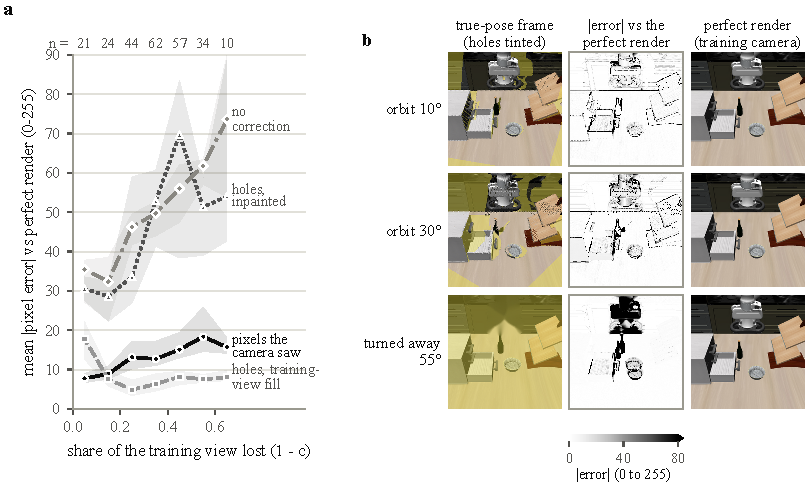
\includegraphics[width=\linewidth]{figs/fidelity.pdf}
\caption{Where the corrected frame is wrong (Prop.~\ref{prop:cov}, Remark~\ref{prop:r3cov}). (a) Error against a perfect
training-view render over the 264 task-placements (median and IQR per bin of lost view; $n$ placements per bin above the
axes; the 12 placements with more than 70\% of the view lost are omitted), split into pixels the camera saw and hole
pixels. With a training-view fill the holes are cheap (median 7.6, mean absolute pixel error on 0 to 255); filling them
by inpainting instead costs several times more and grows with lost view; the error that grows with lost view under the
training-view fill sits on the seen pixels. (b) Three cameras (rows) at the true pose, as in (a): the re-rendered frame
with holes in yellow, its absolute error against the perfect render (0 to 80 shown), and the perfect render. Row 3
(turned away 55 degrees) keeps nothing of the training view at the true pose (a regime (a) omits); its measured pose is
108.9 cm off, so its self-measured coverage 0.71 is not meaningful.}
\label{fig:fidelity}
\end{figure}

\paragraph{The product form of the score\ph.}

\paragraph{Why a product\ph.} Repair is helped by two events: $E_1$, the calibration error falls below the policy's
tolerance, whose probability Prop.~\ref{prop:r2cheb} bounds below by an increasing function of $\ident$ (the
probability itself need not be monotone); and $E_2$, the restored fraction exceeds what the policy needs, which
Remark~\ref{prop:r3cov} makes harder as $c$ falls (the coverage-repair relation itself is empirical,
Fig.~\ref{fig:envelope}b). Without an independence assumption the joint probability is only constrained by the
Fr\'echet bounds, and repair can also happen outside $E_1 \cap E_2$:
\begin{equation}
\begin{gathered}
\max(0, P_1 + P_2 - 1) \le \Pr(E_1 \cap E_2) \le \min(P_1, P_2), \\
\Pr(\text{repair}) = \Pr(E_1\cap E_2)\,\Pr(\text{success} \mid E_1, E_2) + \Pr(\text{repair},\ \overline{E_1\cap E_2}),
\end{gathered}
\label{eq:r3frechet}
\end{equation}
with $P_i = \Pr(E_i)$ (the bounds follow from $\Pr(E_1\cup E_2) \le 1$ and $E_1\cap E_2 \subseteq E_i$; the
decomposition is the law of total probability). The product $\ident \times \invert$ is therefore a heuristic ranking,
not a probability; it equals $P_1P_2$ only under independence and only if its factors are those probabilities.
\emph{Check} (the 98 raw failures of Fig.~\ref{fig:envelope}b; $E_1 =
\{\text{error} \le 2\ \text{cm}\}$, $E_2 = \{\hat c \ge \text{median}\ 0.631\}$). $E_1\cap E_2$: 27, $E_1$ only 22,
$E_2$ only 22, neither 27; $P_1 = P_2 = 0.50$, $\Pr(E_1 \cap E_2) = 0.276$ against the independence value 0.25
(Fr\'echet range $[0, 0.50]$); Fisher exact $p = 0.42$ (odds ratio 1.51). On all 234 camera tasks with both logged,
$p = 0.43$ (odds ratio 1.27). So the rows show no detectable association between the two events, and do not establish
independence either. The decomposition (\ref{eq:r3frechet}) on the 98 failures: $\Pr(\text{repair}) = 0.551 = 0.276
\times 0.926 + 0.296$; repair given both events is 0.93, but more than half of the repairs fall outside $E_1\cap E_2$ at
these thresholds, so the two events are not necessary for repair. \emph{The Fr\'echet upper bound as a score}
(Table~\ref{tab:score} units): $\min(\ident, \invert)$ has AUROC 0.828 [0.72, 0.92] (OFT, 65 units), 0.795 [0.68, 0.90]
(\pihalf, 72) and 0.678 [0.53, 0.82] (OpenVLA, 60), against 0.823, 0.809, 0.675 for the product; paired differences,
product minus minimum, $-0.005$ [$-0.03$, $0.02$], $+0.014$ [$-0.01$, $0.04$], $-0.003$ [$-0.02$, $0.01$]
(unit bootstrap). The combination rule does not matter on these units; the ranking is carried by $\invert$.
The product beats $\ident$ alone on OFT and \pihalf{} (intervals exclude 0) and numerically on OpenVLA ($+0.16$
[$-0.00$, $0.32$]), and ties $\invert$ alone (Table~\ref{tab:score}; paired difference on \pihalf{} $-0.01$ [$-0.10$,
$0.07$]).

\subsection{Remark~\ref{thm:static}: the motion-free test}
\label{app:moreprops}

\paragraph{Full statement of Remark~\ref{thm:static}.}
Assume the body model is exact and the sensing and encoder errors are bounded, so that $\nu_{\max} = \sup
r(q;\eta_0) < \infty$ (supremum over error realisations with the camera at $\eta_0$; see Prop.~\ref{prop:switch} for
unbounded noise). If the camera is at $\eta_0$, the silhouette residual $r(q)$ (Eq.~\ref{eq:resid}) between the
observed mask and the mask rendered at $\eta_0$ at the encoder reading $q$ is a function of sensing and encoder error
alone. A residual that exceeds $\nu_{\max}$ implies $\eta \ne \eta_0$; with an estimated floor this is a test whose
error rates Proposition~\ref{prop:switch} bounds. One pose does not identify $\eta$, but it decides whether
identification is needed.

\paragraph{Remark~\ref{thm:static}.} With $\eta = \eta_0$ and an exact body model, the rendered and observed
silhouettes are the same function of $q$, so $r(q)$ is a function of sensing and encoder error alone and every
realisation has $r \le \nu_{\max}$ by definition of the supremum; the contrapositive is the claim. The test is
one-sided: a zero residual at one pose is consistent with a small set of poses that project the arm identically at that
$q$, which is why the method measures with several poses once the test fires.

\paragraph{Error rates of the motion-free switch\ph.}

\begin{proposition}[separation gives the error rates]
\label{prop:switch}
Model the residual (\ref{eq:resid}) as $r = r_{\mathrm{geo}}(\eta) + e$, where $r_{\mathrm{geo}}(\eta_0) = 0$, the
shifts of interest satisfy $r_{\mathrm{geo}}(\eta) \ge \rho > 0$, and the sensing error $e$ is independent of
$r_{\mathrm{geo}}$ and has the same law under $\eta_0$ and under a shift, with mean $\mu$ and variance $s^2$. For the rule ``measure iff $r > \tau$'' with
$\mu < \tau < \rho + \mu$:
\begin{equation}
\Pr(\text{false alarm}) \le \frac{s^2}{s^2 + (\tau - \mu)^2}, \qquad
\Pr(\text{miss}) \le \frac{s^2}{s^2 + (\rho + \mu - \tau)^2} .
\label{eq:cantelli}
\end{equation}
The larger bound is smallest at $\tau^\star = \mu + \rho/2$, where both equal $s^2 / (s^2 + \rho^2/4)$. If instead
$|e| \le \nu$ almost surely and $\rho > 2\nu$, every $\tau \in [\nu, \rho - \nu)$ has zero error. Finally, if $n_0$
unshifted and $n_1$ shifted units are all classified correctly, the exact one-sided $1 - \alpha$ upper confidence limits
on the two per-unit error rates are $1 - \alpha^{1/n_0}$ and $1 - \alpha^{1/n_1}$.
\end{proposition}

\begin{proof}
A false alarm is $e > \tau$, i.e.\ $e - \mu > \tau - \mu > 0$, and Cantelli's inequality $\Pr(X - \mathbb{E}X \ge
\lambda) \le \mathrm{Var}X/(\mathrm{Var}X + \lambda^2)$ gives the first bound. A miss is $r_{\mathrm{geo}} + e \le
\tau$, which implies $e - \mu \le \tau - \rho - \mu < 0$; Cantelli applied to $-e$ gives the second. The bounds are
decreasing in $\tau - \mu$ and in $\rho + \mu - \tau$ respectively, so the larger is minimised where the two
arguments are equal, $\tau - \mu = \rho/2$. Under $|e| \le \nu$: unshifted $r \le \nu \le \tau$, shifted $r \ge \rho -
\nu > \tau$. With $n$ independent units and error rate $\epsilon$, $\Pr(\text{no error}) = (1-\epsilon)^n$, which is
$\le \alpha$ iff $\epsilon \ge 1 - \alpha^{1/n}$ (the Clopper-Pearson limit for zero events).
\end{proof}

The additive model is the assumption that carries the proposition: the chamfer is not a metric, and the bound holds
for the residual only insofar as sensing error adds to the geometric residual rather than interacting with it. The
bounds are statements about the population moments; with $\mu$ and $s$ estimated from rows they are plug-in values, not
confidence statements, and the equal-law and independence assumptions under a shift cannot be checked from unshifted
rows (untested).

\emph{Check.} \emph{Graded sweep, simulator masks, one pose}: the
60 unshifted units (10 nominal, 50 light) read exactly $0$, so $\nu = 0$; the 70 camera-shifted units read at least
$\rho = 1.929$ (orbit $10^\circ$), median 6.45. The zero-error interval is $[0, 1.929)$ and contains $\tau = 1.5$; the
95\% limits are $1 - 0.05^{1/60} = 0.049$ and $1 - 0.05^{1/70} = 0.042$. The 170 \pihalf{} sweep units of the
motion-free variant read at most 0.020. \emph{LIBERO-Plus, simulator masks} (the pose-averaged statistic $S$ of Eq.~\ref{eq:calnom}, not the one-pose
$r$): the 132 unshifted tasks read at
most $\nu = 0.015$ and the 191 camera-shifted tasks (distinct task ids) at least $\rho = 3.018$; the 95\% limits are
$0.022$ and $0.016$. \emph{Learned masks} (the learned-sensing rows of the same files), where the noise floor is
real: 21 unshifted rows (all joint-offset conditions) have $\mu = 0.567$, $s = 0.162$ (sample standard deviation), maximum
$0.906$. Taking $\rho = 3.018$ from the simulator rows, the plug-in values of (\ref{eq:cantelli}) for statistic $S$ (not
the one-pose $r$; $\mu$ and $s$ from the joint-offset rows) at $\tau = 1.5$ are a false-alarm bound of $0.029$ and a
miss bound of $0.006$; $\tau^\star = 2.08$ would give $0.011$ for both. The
bounded-noise interval with $\nu = 0.906$ is $[0.906, 2.112)$ and contains the post hoc $\tau = 1.5$; the 14 shifted
learned rows read at least $4.85 \ge \rho - \nu$, and all 35 learned rows are classified correctly (95\% limits $0.133$
and $0.193$ at these sample sizes). The sweep's one-pose residual and the
LIBERO-Plus multi-pose score differ in scale because the latter averages over poses at which a shifted camera sees the
arm from further off.

\begin{figure}[tb]
\centering
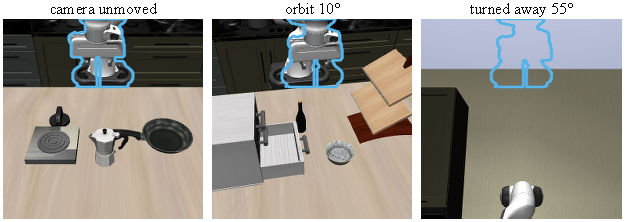
\includegraphics[width=0.75\linewidth]{figs/static_check.pdf}
\caption{The motion-free test of Remark~\ref{thm:static}: the robot's silhouette as the training camera would see it
at the current joint state (blue outline) over the deployed frame, from one rest pose with no arm motion. Camera
unmoved: it lands on the arm (residual 0.00 px) and the probe motion is skipped. Orbit 10 degrees: it misses the arm by
a few pixels (2.08 px, above $\tau = 1.5$), so the robot measures. Turned away 55 degrees: 43.16 px.}
\label{fig:static}
\end{figure}

\subsection{The attribution ladder}
\label{app:ladderproof}

\paragraph{The attribution ladder\ph.}

\begin{proposition}[well-posedness and misattribution]
\label{prop:ladder}
Let the rungs be nested, each changing the previous rung's frame only by making one more component exact (measured
to true pose; reprojection to the training camera's render), and let $Y_k(u)$ be the outcome rung $k$ would have
without rollout noise. \textbf{(a)} Rule (\ref{eq:bucket}) assigns every raw failure to exactly one bucket, whatever
the outcomes. With $S_k$ the number of raw failures that succeed on rung $k$ and $n_j$ the bucket counts, exactly
\begin{equation}
\sum_{j \le k} n_j - S_k = \#\{u : \beta(u) \le k,\ X_k(u) = 0\}, \qquad k = 1,2,3,
\label{eq:ladderid}
\end{equation}
so under monotonicity (M), $Y_1 \le Y_2 \le Y_3$ (making a component exact never turns a noise-free success into a
failure), the noise-free buckets are the increments $n^*_k = S^*_k - S^*_{k-1}$ ($S^*_0 = 0$, $k \le 3$) and a non-monotone observed pattern
certifies at least one flipped rollout. \textbf{(b)} If on every unit each rung's observed outcome differs from $Y_k$ with probability
at most $f$, the observed bucket differs from the noise-free one $\beta^*(u)$ with probability at most
$\min(\beta^*(u), 3)\, f$, with no independence assumption, so the expected number of misattributed units is at most
$f \sum_u \min(\beta^*(u), 3)$. \textbf{(c)} If in addition the flips are independent across rungs and units, each unit with
$\beta^* = 4$ is observed in the policy bucket with probability at least $(1-f)^3$; if $O$ units are observed there,
the one-sided $1-\alpha$ upper confidence limit on their true number is the largest $n$ with
$\Pr\big(\mathrm{Bin}(n, (1-f)^3) \le O\big) \ge \alpha$.
\end{proposition}

\begin{proof}
(a) $\beta$ is a minimum over a finite set with a default, hence a function; the buckets are its level sets. For
(\ref{eq:ladderid}): $\sum_{j\le k} n_j = \#\{\beta \le k\}$, and every unit counted in $S_k$ has $\beta \le k$ by
definition of the minimum, so the difference counts exactly the units with $\beta \le k$ that fail rung $k$. Under
(M) and without noise, $X = Y$ is monotone, the right-hand side is 0, and $n^*_k = S^*_k - S^*_{k-1}$; conversely an
observed pattern with $X_j = 1$, $X_k = 0$, $j < k$, contradicts (M) for $Y$, so $X \ne Y$ on some rung.
(b) If $X_k = Y_k$ for every $k \le \min(\beta^*, 3)$, then for $\beta^* \le 3$ rungs $1, \dots, \beta^* - 1$ fail and
rung $\beta^*$ succeeds, so $\beta = \beta^*$, and for $\beta^* = 4$ rungs 1 to 3 fail, so $\beta = 4$. The event
$\beta \ne \beta^*$ is therefore contained in the union of $\min(\beta^*,3)$ flip events; the union bound and linearity
of expectation give the claims. (c) A unit with $\beta^* = 4$ has $Y_1 = Y_2 = Y_3 = 0$ and is observed as ``policy''
iff none of the three rungs flips, probability $\ge (1-f)^3$ under independence (across rungs and units); $O$ then stochastically dominates
$\mathrm{Bin}(n_{\mathrm{pol}}, (1-f)^3)$, and inverting the binomial tail gives the limit.
\end{proof}

A flip on rung 0 changes which units enter the ladder, not their bucket; it is bounded by the same $f$ per unit. For
a deterministic policy a ``flip'' is the sensitivity of the outcome to the small state and observation differences
between rollouts, which the proposition models as random.

\emph{Check} (set A, all rungs on all tasks).
Success counts 13, 19, 21, 27 and buckets $n = (7, 2, 8, 0)$ reproduce Table~\ref{tab:ladder}. Among the 17 raw
failures $S = (7, 8, 14)$ against cumulative buckets $(7, 9, 17)$; the differences $0, 1, 3$ are exactly the
non-monotone units of (\ref{eq:ladderid}) (task 803: pattern $0,1,0,0$; 800: $0,1,1,0$; 1065: $0,0,1,0$). One raw
success (task 889) is broken by the measured rung and restored by the upper rungs; on the other four OFT sets the upper
rungs were run only on raw failures, so no raw success is broken there by them, and the measured rung breaks 17 more
(18 of 140 in all). For $f$ we
use the only single-rollout flip rate measured on this family: OFT sweep episodes whose outcome changed between raw and
wrapped with nothing applied, 7 of 53 (standard
conditions), $\hat f = 0.132$, one-sided 95\% limit $0.234$; it includes the sweep's arm motion, which all of rungs 1 to 3
share, so it overstates the noise between rungs; and a raw/wrapped discordance of two rollouts that each flip with
probability $f \le 1/2$ occurs with probability $2f(1-f) \ge f$, so $\hat f$ overstates $f$ again. Two caveats: (b)
needs a bound $f$ on every unit, and $\hat f$ is an average over a different task set (the sweep's base tasks); and the
sums below are evaluated at the observed buckets in place of the noise-free ones, so they are plug-in estimates, not
bounds. Plugging the observed buckets into (b): at most
$0.132 \times 35 = 4.6$ of the 17 units are misattributed in expectation on set A, and at most
$0.132 \times 161 = 21$ of the 100 pooled units (buckets 61, 17, 21, 1, so $61 \cdot 1 + 17 \cdot 2 + (21 + 1)
\cdot 3 = 161$). The bucket shares are
therefore uncertain at the level of tens of units; the policy bucket is not: with $O = 1$ observed of 100, (c) gives at
most 5 true policy failures at $\hat f$ and 8 at its upper limit (one-sided 95\% limits given $f$; the uncertainty in
$f$ is covered only by using its upper limit, so by a union bound the statement ``at most 8'' holds at joint one-sided
level at least 90\%, assuming the sweep's $f$ bounds $f$ on every ladder unit). Of the pooled calibration errors (Fig.~\ref{fig:ladder}b), 13 of the 14
only-true-pose OFT units with a logged error exceed 2 cm (median 39.4 cm); of the 19 only-render OFT units with a
logged error, 9 are within 2 cm and 10 exceed it (6 exceed 20 cm; median 2.2 cm); of the 51 OFT units first repaired
at the measured pose with a logged error, 19 exceed 2 cm and 10 exceed 20 cm (logged calibration errors of the measured rung, joined to the buckets of Eq.~\ref{eq:bucket}).

\begin{figure}[tb]
\centering
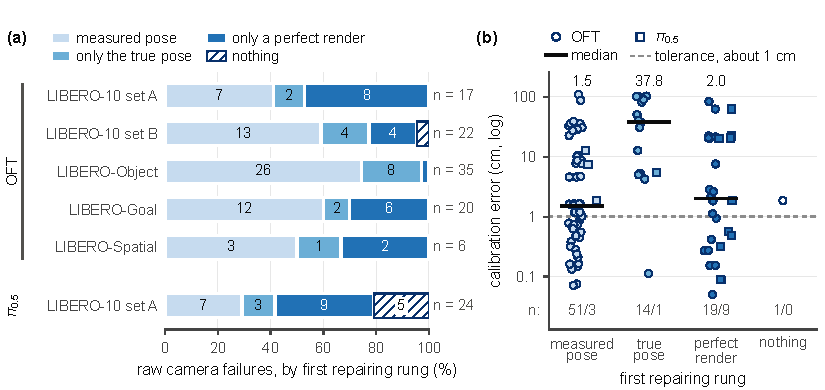
\includegraphics[width=1.0\linewidth]{figs/ladder.pdf}
\caption{All rungs use the simulator's segmentation and depth. (a) Every raw camera failure attributed to the first rung that repairs it (first repaired at the measured
pose; only the true pose; only a perfect render; nothing; light to dark blue, ``nothing'' hatched), per source; rows 1 to 5 are
OFT, row 1 is set A and repeats Table~\ref{tab:ladder}. Pooled over the five OFT rows, 61, 17, 21 and 1 of 100; on the
held-out \pihalf, 7, 3, 9 and 5 of 24. (b) Calibration error of the measured pose per bucket (OFT circles, \pihalf{}
squares; $n$ per strip, OFT / \pihalf: 51 / 3, 14 / 1, 19 / 9, 1 / 0, 98 units with the error logged; bars and numbers
above: medians, none for a single unit; dashed: 1 cm, the action-level tolerance on mild orbits$^\dagger$): units only
the true pose repairs are gross calibration failures (median 37.8 cm; OFT alone 39.4 cm); units only a render repairs
have median error 2.0 cm (OFT alone 2.2 cm, but 10 of its 19 exceed 2 cm).}
\label{fig:ladder}
\end{figure}

\FloatBarrier
\section{Registered tests and their outcomes}
\label{app:prereg}
Each test below was written to a dated log, with its constants and pass criteria, before any data that could test it
existed. Development-family (OFT) outcomes are descriptive; held-out outcomes are the test.

\begin{table}[!ht]
\centering\small
\caption{Registered tests and their outcomes. Every test was written to a dated log, with its constants and pass criterion, before any data that could test it existed. H-F1 to H-F5 test the action-fingerprint selector (fingerprint distance,
App.~\ref{app:defs}); the H-F2 values are the registered raw-frame statistic.}
\label{tab:prereg}
\resizebox{\linewidth}{!}{%
\begin{tabular}{p{3.6cm}p{5.2cm}p{5.6cm}}
\toprule
test (registered) & rule & outcome \\
\midrule
Recoverability score as a predictor (frozen 2026-09-17) & rank raw failures by $\recover$; no numeric bar registered &
descriptive; no pass criterion was registered: 0.809 [0.69, 0.91] (\pihalf), 0.675 [0.52, 0.82] (OpenVLA).
Post hoc note\ph: both above the category label (0.515, 0.472) \\
Do-no-harm gate (2026-09-18) & veto a correction if the action changes more under benign jitters of the corrected frame
than of the raw one & \textbf{fails}: over 386 paired gated / ungated units on the two held-out families it vetoed 49,
saved 1 unit and broke 16 ($p = 3\times10^{-4}$); where it does not veto it reproduces the ungated variant exactly \\
Score-gated correction (2026-09-19) & correct the camera only if coverage $\ge 0.5$ & \textbf{killed} by its own
criterion on rows unseen when frozen: prevented 2 breaks, gave up 3 repairs \\
Ray-concurrency probe (2026-09-19) & triangulate a sub-goal from 7 probe actions & \textbf{fails} on both families
(AUROC 0.32 to 0.56) \\
Action-field fingerprint, H-F1 to H-F5 (amendment, 2026-09-19, before any held-out probe) & H-F1 corrected AUROC
$\ge 0.80$; H-F2 raw AUROC $\ge 0.70$; H-F3 keep raw on $\ge$ half the units a correction breaks; H-F4 keep the
correction on $\ge 80\%$ of units it repairs; H-F5 selected success $\ge$ best fixed variant minus one unit & \pihalf:
H-F3 and H-F5 pass (5 of 5; 0.86 against 0.81), H-F1 0.787, H-F2 0.684, H-F4 7 of 9 narrowly fail. OpenVLA:
H-F1 0.643, H-F2 0.659, H-F4 3 of 13, H-F5 0.32 against 0.46 fail; H-F3 undetermined (one unit) \\
DROID self-calibration stop rule (written before the final calibration run) & stop if the median error on reliable references exceeds 30 cm &
\textbf{fired} (32.1 cm); the later mask change reaching 19.6 cm is post hoc (Appendix~\ref{app:droid}) \\
Replication on 6 unseen OpenVLA base tasks (frozen 2026-09-25, before any row) & deployable
score (self-measured $\ident$, residual gate $\tau = 0.547$): H1 within-category AUROC $> 0.5$ (within-category
permutation, one-sided 0.05); H2 same, pooled with the 60 registered units; H3 residual flags calibration failure,
AUROC $\ge 0.90$; H4 AUROC within 0.05 of the registered score & \textbf{all pass} (3 of 6 tasks solved, 52 units,
22 repaired): H1 0.663, $p = 0.036$; H2 0.655, $p = 0.007$; H3 1.000 (21 units, 10 failures); H4 0.667 vs 0.615 \\
Learned sensing + refined pose, closed loop, OFT set A (frozen 2026-09-25, before any row) & H5 success above raw
(one-sided exact McNemar, 0.05); H6 wins $\ge$ losses against the earlier learned pipeline & H5 \textbf{fails} (19 vs
15; 6 repaired, 2 broken, $p = 0.14$); H6 \textbf{passes} (19 vs 12; 7 wins, 0 losses) \\
Refined pose on \pihalf, 60 camera tasks (same file) & H7 success above raw (one-sided exact McNemar, 0.05); H8 the
same for the unrefined correction & H7 \textbf{passes} (15 repaired, 3 broken, $p = 0.004$); H8 passes over all 60 (15
and 6, $p = 0.039$), not on the 30 new tasks alone (8 and 4, $p = 0.19$) \\
Learned sensing + refined pose on OFT set B and on \pihalf{} (frozen 2026-09-26) & H9, H11
success above raw; H10, H12 within 3 tasks of simulator sensing & Not run before submission \\
\bottomrule
\end{tabular}}
\end{table}

\FloatBarrier
\section{Additional results}
\label{app:extra}

\subsection{The recoverability score}

\paragraph{Score: first test and task-cluster intervals.} The first score test used three base tasks per family
(Table~\ref{tab:first}). Task-cluster bootstrap intervals for Table~\ref{tab:score}: OFT [0.73, 0.92], \pihalf{} [0.66,
0.94], OpenVLA [0.59, 0.82] (3 solved base tasks, so its cluster interval is unreliable). Against the category rate fit
on OFT, the paired score difference on \pihalf{} is $+0.109$ (unit bootstrap [$-0.03$, $0.24$], task-cluster [$-0.03$,
$0.25$]) and on OpenVLA $+0.061$ [$-0.10$, $0.22$]; against the label $+0.294$ [$0.18$, $0.39$]; against $\ident$ alone
$+0.183$ [$0.09$, $0.30$]; against $\invert$ alone $-0.010$ [$-0.10$, $0.07$]. A finer baseline\ph, the repair rate per
\emph{condition} fit on OFT, reaches 0.745 on \pihalf, and the score minus it is $+0.077$ [$-0.02$, $0.19$]: the score is
not shown to be the best category-based predictor, only numerically above both. Shift magnitude, where defined, gives
0.29 (translation, $n=45$) and 0.82 (rotation, $n=45$) on \pihalf. The look-away units are shown against the score in
Fig.~\ref{fig:tilt}. Units are (base task, condition), one rollout each (no key
repeats in the sweep rows, so no averaging occurs). Across categories $\ident$ gains about 0.04 by demoting negatives
and gives back as much on repaired units, so the pooled score ties $\invert$ alone. On look-away units $\ident$ is below
1 on 11 of 18 on \pihalf{} and OFT (3 of 6 on OpenVLA), its net pair contribution there is $+0.018$ on OFT and
$-0.005$ on \pihalf, and OFT repairs 2 of 18, OpenVLA 0 of 6. A registered rule that corrected the camera only at
coverage $\ge 0.5$ failed its pre-stated criterion (2 breaks prevented, 3 repairs lost; App.~\ref{app:prereg}).

\paragraph{The deployable score\ph.} (Units of
Table~\ref{tab:score}; non-camera units unchanged; task-cluster intervals.) AUROC on OFT, \pihalf, OpenVLA and
within-category on the pooled held-out families:
registered (true-pose $\ident$) 0.823, 0.809, 0.675, 0.737 [0.64, 0.87];
true-pose $\ident$ recomputed in the rescoring run 0.826, 0.805, 0.671, 0.730;
self-measured $\ident$, no gate 0.765, 0.773, 0.666, 0.679 [0.57, 0.81];
self-measured $\ident$ with the residual gate 0.802 [0.68, 0.91], 0.837 [0.73, 0.93], 0.691 [0.62, 0.82], 0.713 [0.60,
0.84]. Calibration failure ($> 2$ cm) on the 119 camera units with a logged calibration: the residual $\rho$ has AUROC
1.000 on each family; the gate flags 12 of 12 OFT, 36 of 36 \pihalf{} (one false alarm of 34) and 8 of 8 OpenVLA
failures (none of 20). The self-check F1 is logged on 53 of the 119 units and is weaker (0.614). Under learned masks
and monocular metric depth (set A, 30 units) the same $\tau$ separates the one fit within 2 cm from all 29 beyond. On
real DROID images (53 calibrations, VLM-chosen masks) the residual is weaker: it ranks
calibrations beyond 10 cm at AUROC 0.71 [0.50, 0.88] and beyond 20 cm at 0.60 [0.44, 0.76], so the gate is not shown to
transfer to real images.

\paragraph{Within-category ranking\ph.} (same units; cluster bootstrap over
base tasks, 2{,}000 resamples, seed 0.) A predictor constant within a stratum has AUROC exactly $\tfrac12$ over
(repaired, unrepaired) pairs drawn from the same stratum, so the stratified AUROC
$A_{\mathrm{strat}}(s) = \sum_g \#\{(i,j) \in g: i \text{ repaired}, j \text{ not}, s_i > s_j\} / \#\{\text{such pairs}\}$
(ties one half) measures only what a predictor adds on top of any category router. Over same-category pairs (OFT 366,
\pihalf{} 502, OpenVLA 132) the score reaches 0.794 [0.62, 0.94], 0.854 [0.75, 0.96] and 0.720 [0.50, 0.85], and 0.737
[0.64, 0.87] pooled over the held-out families; $\invert$ alone 0.709, 0.761, 0.693 (0.684 pooled); $\ident$ alone
0.661, 0.656, 0.614. Paired within-category differences (cluster bootstrap): score minus $\ident$ $+0.151$ pooled
held-out (one-sided $p = 0.001$), significant on every family except OpenVLA; score minus $\invert$ $+0.093$ on
\pihalf{} ($p = 0.035$), $+0.053$ pooled held-out ([$-0.02$, $+0.14$], $p = 0.079$), $+0.027$ on OpenVLA (n.s.).
Within a single condition there are too few pairs (148 pooled held-out) to conclude anything.

\paragraph{Stronger baselines\ph.} (unit bootstrap, 2{,}000 resamples, seed 0; paired
differences on the same units.) $\min(\ident, \invert)$ matches the product on every family (OFT 0.828 against 0.823;
\pihalf{} 0.795 against 0.809; OpenVLA 0.678 against 0.675; paired differences within $\pm0.04$; App.~\ref{app:proofs},
``Why a product''). On \pihalf{} camera units the true rotation magnitude reaches 0.818 [0.68, 0.93] against the
score's 0.877 on the same 45 units (score minus it $+0.059$ [$-0.05$, $0.18$]): it ties the score. True-pose coverage
and a true-pose image statistic are logged only policy-free, on the three envelope
base tasks, which leaves 12 to 18 units per family (OFT: true-pose coverage 0.806 against the score's 0.861 on the same
12 units), too few to rank. No image statistic of the corrected frame the wrapper actually fed the policy (pixel error
or SSIM against the training reference) is logged in any rollout row, so that baseline cannot be computed from the rows. On the 98 in-rollout camera failures of Fig.~\ref{fig:envelope}b,
coverage beats translation (paired $+0.222$ [$0.07$, $0.38$]) and is numerically above rotation ($+0.085$ [$-0.01$,
$0.19$], same bootstrap).

\paragraph{Baselines on set B.} Table~\ref{tab:baselines} runs every method on every task of set B. Test-time
augmentation (TTA) breaks nothing, but over 150 camera tasks on three suites the wrapper beats it on 46 tasks and loses
on 13 ($p<10^{-4}$), and TTA alone does not beat the raw policy on LIBERO-Object or LIBERO-Goal.

\paragraph{Why the weaker family scores lower\ph.} On OpenVLA, 5 of its 24 repaired units had \emph{no channel applied}
(OFT: 0 of 37; \pihalf: 1 of 37): the measurement's arm motion jostled a fragile policy into success, and four of the
five are background units at $\recover = 0$. With $P$ repaired units, $m$ of them of this kind, and $\widehat
A_{\mathcal G}$, $\widehat A_{\mathcal C}$ the AUROC on the other and on these positives, the AUROC is exactly
$\widehat A = \tfrac{P-m}{P}\widehat A_{\mathcal G} + \tfrac{m}{P}\widehat A_{\mathcal C}$,
and these units take 0.816 to 0.675, to the digit. Redefining the outcome symmetrically, $\mathrm{repaired}^*(u) =
\mathrm{repaired}(u) \wedge \text{(some channel applied)}$, and dropping every unit where nothing was applied, gives
0.817 ($n = 64$), 0.826 (70) and 0.782 (49) (one-sided exclusion: 0.823, 0.831, 0.816): the gap to the best family
shrinks from 0.15 (0.823 vs 0.675) to 0.04 (0.826 vs 0.782). The registered result stays 0.675.

\paragraph{Level-5 tasks.} On LIBERO-Plus level-5 tasks (the hardest grade), the servo repairs 32 of 33
robot-initial-state failures, and coverage still ranks level-5 camera failures (AUROC 0.75, $n = 47$).

\begin{table}[h]
\centering\small
\caption{The first score test, three base tasks per family (the setting in which the score was first frozen).}
\label{tab:first}
\begin{tabular}{lcccc}
\toprule
 & units & repaired & AUROC, score & AUROC, label \\
\midrule
OFT (development) & 21 & 14 & 0.908 [0.68, 1.00] & 0.500 \\
\pihalf{} (held out) & 21 & 14 & 0.837 [0.64, 1.00] & 0.464 \\
pooled & 42 & 28 & 0.881 [0.76, 0.98] & 0.482 \\
\bottomrule
\end{tabular}
\end{table}

\begin{table}[h]
\centering\small
\caption{Baselines on set B, the 30 LIBERO-10 camera tasks after the first 30 (OFT; 22 raw failures, 8 raw successes),
every method on every task; disjoint from set A (Table~\ref{tab:ladder}). The measured pose without depth, generic fixes
and test-time augmentation all lose to the wrapper.}
\label{tab:baselines}
\begin{tabular}{lcccc}
\toprule
method & success & repaired & broken & wrapper wins / losses, $p$ \\
\midrule
raw policy & 0.27 & & & \\
generic fixes (WB, CLAHE, denoise) & 0.37 & 3/22 & 0/8 & 10 / 2, 0.039 \\
homography, no depth & 0.40 & 9/22 & 5/8 & 9 / 2, 0.065 \\
TTA & 0.47 & 6/22 & 0/8 & 8 / 3, 0.23 \\
\textbf{wrapper} & \textbf{0.63} & 13/22 & 2/8 & \\
\bottomrule
\end{tabular}
\end{table}

\begin{table}[h]
\centering\small
\caption{Secondary paired tests and Holm-adjusted $p$ over the $m = 15$ secondary tests, one row per test, ordered by
raw $p$ (step-down, monotone). The three task-level rows use the exact sign-flip test
(Eq.~\ref{eq:signflip}): the motion-free row over the 7 tasks with a non-zero difference (the episode-level McNemar is
0.0125, Holm 0.088 in that family), the two replicate rows over 3 replicates; all other rows use the exact McNemar test
(Eq.~\ref{eq:mcnemar}), or Wilcoxon where stated. Primary: pooled OFT camera, 61 of 100 repaired, 18 of 140 broken, $p =
1.3\times10^{-6}$.}
\label{tab:holm}
\begin{tabular}{lccc}
\toprule
comparison & repaired / broken & $p$ & Holm $p$ \\
\midrule
OFT joint, three untuned suites & 47 / 1 & $3.5\times10^{-13}$ & $5.2\times10^{-12}$ \\
OFT Object joint & 16 / 0 & $3.1\times10^{-5}$ & $4.3\times10^{-4}$ \\
OFT Goal joint & 16 / 0 & $3.1\times10^{-5}$ & $4.3\times10^{-4}$ \\
\pihalf{} joint & 16 / 0 & $3.1\times10^{-5}$ & $4.3\times10^{-4}$ \\
OFT LIBERO-10 joint & 18 / 1 & $7.6\times10^{-5}$ & $8.4\times10^{-4}$ \\
OFT LIBERO-10 camera & 20 / 3 & $4.9\times10^{-4}$ & 0.0049 \\
OFT Spatial joint & 15 / 1 & $5.2\times10^{-4}$ & 0.0049 \\
OFT Object camera & 26 / 6 & $5.4\times10^{-4}$ & 0.0049 \\
DROID masks (Wilcoxon)\ph & & 0.015 & 0.11 \\
motion-free vs.\ raw, \pihalf{} sweep, task level\ph & 21 / 7 & 0.047 & 0.28 \\
\pihalf{} light, 3 replicates, task level\ph & 3 / 13 & 0.078 & 0.39 \\
\pihalf{} camera, 3 replicates, task level\ph & 21 / 8 & 0.12 & 0.48 \\
OFT Goal camera & 12 / 5 & 0.14 & 0.48 \\
\pihalf{} camera, one rollout & 7 / 2 & 0.18 & 0.48 \\
OFT Spatial camera & 3 / 4 & 1 & 1 \\
\bottomrule
\end{tabular}
\end{table}

\subsection{Correction and sensing}

\paragraph{Does the stored-view hole fill drive the repairs?\ph} The reprojection fills holes
from a stored training-view image, which could act as a partial oracle. On the 30 OFT set-B camera tasks the no-fill variant, which inpaints the holes from the deployed frame instead, solves 20 against 19 for the evaluated wrapper on the same seeds (fill-only successes 1, no-fill-only 2; exact McNemar $p = 1.0$); on 8 \pihalf{} camera
tasks, 3 against 1. Across the 98 in-rollout camera failures, repair is lowest where the fill dominates: 4 of 19 (21\%)
below coverage 0.5, 29 of 51 (57\%) at 0.5 to 0.7, 15 of 19 (79\%) at 0.7 to 0.85, 6 of 9 at 0.85 and above. The
repairs therefore come from the re-projected geometry, not from the pasted training view.

\paragraph{The residual on learned sensing, in closed loop\ph.} On the 30 learned-sensing
rollouts of set A, the refinement's own final loss ranks the calibrations that failed (beyond 2 cm) at AUROC 0.777.
Acting only when that loss is below a threshold fixed on the policy-free runs beforehand (0.0071, the largest loss of a
fit within 2 cm on sets A and B) repairs 5 and breaks 1, against 6 and 2 without the gate (one-sided $p = 0.11$ and
$0.14$). The gate removes one break at the cost of one repair, which is too small to matter at this sample size.

\paragraph{Task-aware coverage\ph.} Coverage weights
every pixel equally. Restricting it to the task-relevant pixels of the training view (every movable object and the
gripper) and computing it at the true camera pose for the 63 LIBERO-10 ladder camera failures (OFT sets A and B,
\pihalf{} set A), it ranks the failures that a geometric rung repairs at AUROC 0.847, against 0.802 for whole-frame
coverage at the same pose. A rule we fixed beforehand, that task coverage below 0.5 certifies a failure as
unrepairable by any geometric correction, certified none of the 63: even the render-only failures keep a median of 84\%
of their task pixels, so their loss is not a loss of the task pixels themselves.

\paragraph{How good the masks must be\ph.} On 12
set-A camera tasks we took the simulator's masks from the method's sweep and corrupted them at four increasing levels
(boundary pixels flipped with probability one half in a band of 1 to 4 px, plus up to three false-positive blobs and two
holes), then ran the same calibration and two-start refinement with depth from the table plane. The median mask IoU and
median calibration error per level were 1.00 and 1.73 cm, 0.82 and 1.65 cm, 0.68 and 3.31 cm, 0.54 and 9.35 cm, and 0.45
and 8.96 cm, with 7, 7, 4, 0 and 2 of 12 tasks within 2 cm. Calibration therefore holds down to an IoU of about 0.8 and
fails below about 0.6.

\paragraph{Rollout noise on \pihalf.} The three replicated runs of Sec.~\ref{sec:undo} hold the task and the
perturbation fixed and vary the seed (environment and policy sampling seed $=$ task id $+ 1000 \times$ replicate).
Across them the outcome of a task changes on 10\% of camera tasks under the raw policy and 33\% under the measuring
wrapper, the arm-motion mechanism of Sec.~\ref{sec:cost} seen as variance; with the same seed the raw policy changes 0
of 20 outcomes. On the 10 light tasks run alongside, the motion-free variant breaks 1 of 9 raw successes where
measuring always breaks 3 of 9; over the three replicates the measuring wrapper breaks 13 and repairs 3 episodes
(episode-level $p=0.021$). Task-level, with $D_i \in \{-3, \dots, 3\}$ the
summed wrapped-minus-raw difference over the three replicates: \emph{camera}, 30 tasks, histogram $\{-3{:}\,2,\ -1{:}\,1,\
0{:}\,15,\ 1{:}\,6,\ 2{:}\,4,\ 3{:}\,2\}$, so 12 positive, 3 negative, $n_0 = 15$, null size $2^{15} = 32{,}768$,
smallest attainable $p = 6.1\times10^{-5}$; sign test $p = 0.035$, sign-flip $p = 0.119$, Wilcoxon $p = 0.094$.
\emph{Light}, 10 tasks, $\{-3{:}\,2,\ -2{:}\,1,\ -1{:}\,3,\ 0{:}\,3,\ 1{:}\,1\}$, 1 positive, 6 negative, $n_0 = 7$,
$2^7 = 128$, smallest $p = 0.016$; sign $p = 0.125$, sign-flip $p = 0.078$, Wilcoxon $p = 0.078$. The camera tests
differ because the sign test counts only the 12 against 3 signs, while the sign-flip test weights each task by $|D_i|$
and the two tasks at $-3$ weigh heavily against a positive side made mostly of $+1$s; Wilcoxon ranks the magnitudes and
falls between the two.

\paragraph{Ladder buckets: uncertainty and error.} Bucket shares are uncertain at the level of about 21 of 100 units
(App.~\ref{app:moreprops}); the bound of at most 8 policy units holds at joint one-sided level at least 90\% (95\% for
$f$, 95\% given $f$) and is a plug-in estimate. Only-render units have median calibration error 2.2 cm, but 10 of 19
logged exceed 2 cm, and they have the lowest self-measured coverage (render-only against the other two buckets, AUROC
0.81 [0.65, 0.94], task-cluster, $n = 97$\ph). Of the 51 logged measured-rung repairs, 19 exceed 2 cm and 10 exceed 20
cm, so those repairs are not due to reprojection (fill or arm motion) and fall inside the misattribution budget. The
light channel on \pihalf{} shows a harmful trend (3 repaired, 13 broken over three post hoc replicates; task-level $p =
0.078$)\ph; the \pihalf{} camera replicates give sign test $p = 0.035$ and exact sign-flip $p = 0.12$ on the task-level
summed difference.

\subsection{The cost of measuring, and a test that removes it}
\label{sec:cost}
Self-measurement moves the arm, and the held-out \pihalf{} is sensitive to where its episode starts. Over the whole
graded sweep (240 units) the measuring wrapper repairs 44 of 82 \pihalf{} failures and breaks 45 of 158 successes, for
no net gain. The probe motion hands the arm back 10 to 25 mm off and still moving, and this alone changes 15 of 48
outcomes where nothing else was applied (against 0 of 20 on a same-seed rerun; App.~\ref{app:extra}).
Remark~\ref{thm:static} lets the robot avoid the motion\ph. It looks once at its own silhouette without moving and
measures only if the residual exceeds $\tau = 1.5$ px. Otherwise it \emph{settles}, returning the arm to the episode's
start and waiting until it is still.

\begin{figure}[t]
\centering
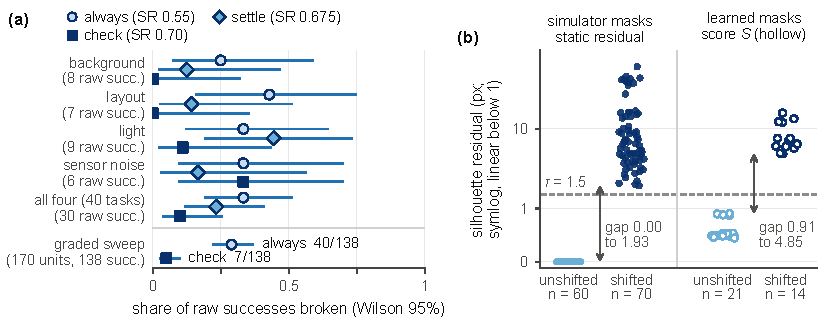
\includegraphics[width=\linewidth]{figs/harm.pdf}
\caption{(a) \pihalf, 40 tasks in four non-camera categories with no correction applied (30 raw successes): share of
raw successes broken (Wilson 95\%) when the wrapper measures always (circle), measures then settles (diamond), or runs
the motion-free check first (square); success rates 0.55, 0.675 and 0.70 (decomposed in App.~\ref{app:extra})$^\dagger$.
Bottom: the 170-unit graded sweep (138 raw successes), where the check never fires and so equals never measuring
(task-level $p = 0.031$ vs.\ measuring always, $0.047$ vs.\ raw)$^\dagger$. (b) Filled: one-pose silhouette residual
(Eq.~\ref{eq:resid}), simulator masks, policy-free: 60 unshifted units (10 nominal, 50 lighting; largest 0.00; 0.020
over the 170 \pihalf{} units) against 70 camera shifts (smallest 1.93). Hollow: learned masks, the pose-averaged score
$S$ (Eq.~\ref{eq:calnom}), a different statistic (21 unshifted OFT rows, largest 0.906; 14 shifted, smallest 4.85).
$\tau=1.5$ chosen post hoc.}
\label{fig:harm}
\end{figure}

The residual separates the two cases on every logged unit (Fig.~\ref{fig:harm}b; App.~\ref{app:moreprops}). With no
error observed on 10 base-task clusters, the one-sided 95\% upper limit on either error rate is 0.259
(exact binomial over clusters). Between the tolerance (under $1^\circ$ of orbit) and about $8^\circ$ of orbit we have not
shown that the check fires. On the 170 sweep units without a camera shift (138 raw successes
and 32 raw failures), where the test should not fire and did not, the measuring wrapper breaks 40 and repairs 25. The
motion-free variant breaks 7 and repairs 21, keeping 18 of the 25 repairs and adding 3 (Fig.~\ref{fig:harm}a; against
measuring always 41 wins and 12 losses, $p = 8.2\times10^{-5}$; against raw 21 and 7, $p = 0.013$; task-level\ph{}
$p = 0.031$ and $0.047$). Where it has to decide\ph{} (\pihalf, 60 rollouts), it fires on all 30 camera tasks (smallest
residual 4.04) and on none of the 30 joint-offset tasks (largest 0.01). It then matches always-measuring on camera (7
of 24 repaired and 2 of 6 broken for both) and stays within noise on joint offsets (14 of 19 and 1 of 11 against 16 of
19 and 0 of 11, $p = 0.38$).

\paragraph{The cost of the measuring motion.} The probe motion hands the arm back 10 to 25 mm from where the episode
began and still moving at 0.19 rad/s; re-running the raw policy with the same environment and sampling seeds changes 0
of 20 outcomes (one-sided 95\% upper bound 14\%; layout and background tasks), against 15 of 48 changed when the arm
moved and nothing else was applied.

\paragraph{The motion-free variant, decomposed\ph.} On the 40 non-camera \pihalf{} tasks of Fig.~\ref{fig:harm}a
(one rollout each) the
success rates are 0.75 (raw), 0.55 (measure always), 0.675 (measure then settle) and 0.70 (motion-free
check first), and
\begin{equation}
\mathrm{SR}_{\mathrm{check}} - \mathrm{SR}_{\mathrm{full}} = (\mathrm{SR}_{\mathrm{check}} - \mathrm{SR}_{\mathrm{settle}})
+ (\mathrm{SR}_{\mathrm{settle}} - \mathrm{SR}_{\mathrm{full}}) = (+0.025) + (+0.125) = +0.150 .
\end{equation}
Exact McNemar on discordant tasks: check vs.\ settle 6 / 5, $p = 1.0$; settle vs.\ full 6 / 1, $p = 0.125$; check vs.\
full 8 / 2, $p = 0.11$; check vs.\ raw 1 / 3, $p = 0.63$. Settling the arm after the probe motion supplies most of the
gain, and on these tasks the check adds nothing measurable over settling. On the graded sweep (170 non-camera units, 10
base tasks, all \pihalf{} shards merged) the per-task differences, check minus measure always, are $D = (3, 10, 0, 4, 0,
6, 0, 2, 4, 0)$: $n_0 = 6$, null size $2^6 = 64$, smallest attainable $p = 0.031$, and the exact sign-flip test
(\ref{eq:signflip}), the sign test and Wilcoxon all give $p = 0.031$ (episode-level McNemar 41 / 12, $p = 8.2\times
10^{-5}$). Check minus raw: $D = (0, -1, 0, 1, 3, 0, 3, 2, 2, 4)$, $n_0 = 7$, $2^7 = 128$, sign-flip $p = 6/128 =
0.047$, Wilcoxon $0.047$, sign test $0.125$ (episode-level 21 / 7, $p = 0.013$). Measure always minus raw: sign-flip $p
= 0.38$. On these units the check never fires, so it is equivalent to never measuring, and its ability to fire rests on
the policy-free separation of Fig.~\ref{fig:harm}b. The largest static residual over the 170 sweep units is 0.020 px
(joint offset 0.20 on task 1442; next 0.019, offset 0.35 on task 1167); 145 of 170 are exactly 0, and all 25 nonzero
values are on units where the arm was servoed to the training start just before the check (11 joint-offset units and
the 14 other units of task 1101, whose start is 0.071 rad off); the model mask is rendered at the encoder reading, not
at a stored rest pose (App.~\ref{app:proofs}).

\subsection{How exact the calibration must be}
\label{app:tolerance}
How precisely must the camera be measured for the frozen policy to act as it did in training? The fingerprint
distance (App.~\ref{app:defs}) answers this without rollouts, as the dose of pose error at which the policy's probe
actions start to change (Fig.~\ref{fig:tolerance}). The knee of the action response moves to 0.5 and 4 cm at thresholds of 0.05 and 0.20, and because the response is sublinear it is bounded by the smallest crossing dose. In-rollout repair rates by calibration error show no knee at 1 cm (App.~\ref{app:extra}).

\begin{figure}[tb]
\centering
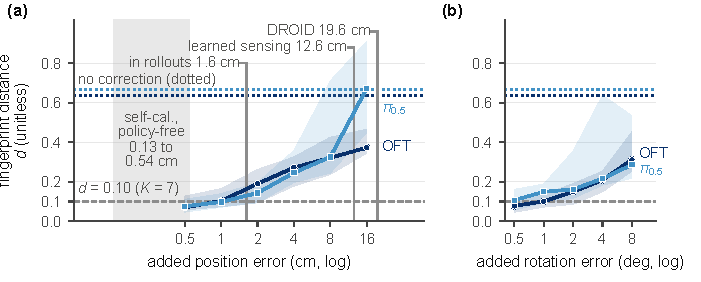
\includegraphics[width=0.85\linewidth]{figs/tolerance.pdf}
\caption{How exact the calibration must be, with no rollouts$^\dagger$. Fingerprint distance $d$ (Eq.~\ref{eq:fp},
$K = 1$: the first action chunk at the episode's untouched start state) between the opening actions at the true camera
pose plus a known (a) position or (b) rotation error and at the true pose (reference: the true-pose corrected frame);
median and IQR over $n = 20$ runs per family (orbit 10 and 20 degrees, coverage $\ge 0.68$, 10 tasks each). Dashed:
$d = 0.10$, the $K = 7$ threshold, drawn for reference only (knees in Sec.~\ref{sec:ladder}). Dotted: no correction.
Grey band: policy-free self-calibration error on 8 tasks (0.13 cm with 7 probe poses to 0.54 cm with 1). Leaders:
median calibration error in the evaluated OFT camera rollouts (1.6 cm, $n = 219$), with learned sensing (12.6 cm,
$n=30$), on real DROID images (19.6 cm, $n=53$).}
\label{fig:tolerance}
\end{figure}

\paragraph{Outcome tolerance in rollouts\ph.} On the 98 in-rollout
camera raw failures of Fig.~\ref{fig:envelope}b (85 OFT, 13 \pihalf, all with the pose applied; 54 repaired), the
repair rate by calibration error is 22 of 34 (0.65 [0.48, 0.79], Wilson) below 1 cm, 11 of 15 (0.73 [0.48, 0.89]) at 1
to 2 cm, 3 of 7 (0.43 [0.16, 0.75]) at 2 to 5 cm, 8 of 13 (0.62 [0.36, 0.82]) at 5 to 20 cm and 10 of 29 (0.34 [0.20,
0.53]) at 20 cm or more. The isotonic (non-increasing) fit is flat at 0.71 up to 1.83 cm, then 0.50, 0.47 and 0.17
beyond 41 cm (breakpoints 1.83, 20.1, 41.0 cm): in rollouts there is no knee at 1 cm, and the action-level tolerance of
Fig.~\ref{fig:tolerance} is a statement about opening actions, not outcomes.

\begin{figure}[tb]
\centering
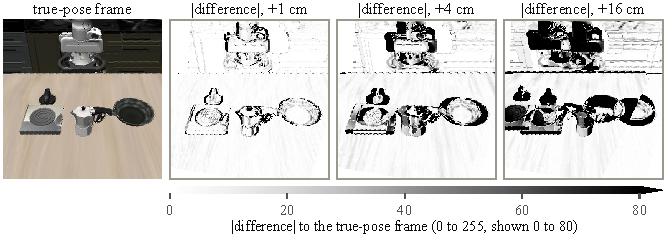
\includegraphics[width=0.8\linewidth]{figs/tolerance_pictures.pdf}
\caption{The tolerance in pixels, on one unit of Fig.~\ref{fig:tolerance} (task 1167, orbit 10 degrees): the true-pose
frame and its absolute difference to the frames at 1, 4 and 16 cm of added position error (mean 7.4, 16.7 and 30.1 on
0 to 255; shown 0 to 80). On this unit the fingerprint distance $d$ at the same doses is 0.078, 0.295 and 0.365 for OFT
and 0.062, 0.158 and 0.182 for \pihalf{} (family medians 0.104, 0.272, 0.373 and 0.099, 0.246, 0.672). At 1 cm the
median opening action has changed by 10\% (the reference threshold), while every edge has moved: pixel difference does
not measure what the policy tolerates, which is why tolerance is measured on actions$^\dagger$.}
\label{fig:tolpics}
\end{figure}

\begin{figure}[tb]
\centering
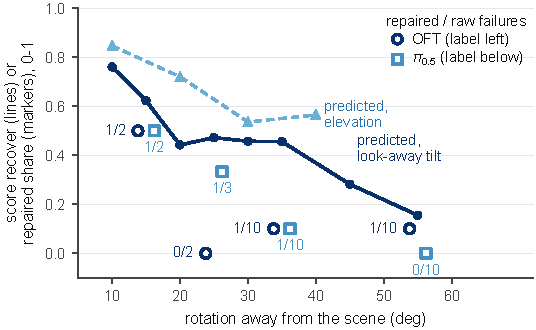
\includegraphics[width=0.65\linewidth]{figs/envelope_tilt.pdf}
\caption{The score as the camera rotates away from the scene (dark blue, solid: look-away tilt; light blue, dashed: elevation; mean over
three base tasks). The policy-free map scores a 35-degree look-away 0.46 on average, while the sweep's own scores at
that condition, from the self-measured pose, average 0.24 over its 10 base tasks. Markers: repaired / raw failures of the
graded sweep at each look-away condition, all ten base tasks (not the Table~\ref{tab:score} prediction units), OFT left
of and \pihalf{} below each marker.}
\label{fig:tilt}
\end{figure}

\paragraph{A nuisance the body does not model.} Zooming the true camera while the wrapper assumes the training focal
length (8 camera tasks, policy-free) is absorbed as a camera that backed away along its own optical axis: at 5, 10 and
20\% zoom the pose error is 2.7, 5.9 and 10.8 cm, almost all of it along that axis. The corrected frame degrades
gracefully (image error 14.5, 16.3 and 20.1 against about 30 uncorrected and 10.2 with the true focal length), and the
self-check barely notices (F1 0.93 to 0.83): it checks the pose it was asked about, not the model behind it. Focal
length is not aliased with the 6-DoF pose (Jacobian residual 0.78 against a median of 0.51 among the pose columns), so
three poses at different depths identify it; lens shift in $x$ is aliased with a 0.44 degree pan, which undoes it.

\paragraph{Figures.} Fig.~\ref{fig:ladder} gives the ladder per source and the calibration error per bucket; rows 3
and 4 of Fig.~\ref{fig:teaser} show the two upper rungs in pictures. Fig.~\ref{fig:tilt} gives the look-away line.
Fig.~\ref{fig:fidelity} tests Prop.~\ref{prop:cov} and Remark~\ref{prop:r3cov}; Fig.~\ref{fig:static} shows the motion-free
test and Fig.~\ref{fig:tolpics} the frames behind the tolerance probe. Over the 88 camera placements $\times$ 3 base
tasks of Fig.~\ref{fig:envelope}a ($\ident = \sigma_{\min}/\sigma_{\min,
\mathrm{ref}}$ capped at 1), $\ident \ge 0.9$ on 199 of the 264 task-placements (at least 0.61 on all 240 that do not
turn away from the scene; minimum 0.18 at a 55 degree look-away), so across the orbit and distance map $\recover$
tracks coverage (Pearson $r = 0.84$ with coverage and $0.03$ with identifiability over the 192 task-placements of the
azimuth-by-distance grid, App.~\ref{app:defs}).

\section{Real images: DROID}
\label{app:droid}
Fig.~\ref{fig:droid} reports the self-calibration on real images.

\begin{figure}[h]
\centering
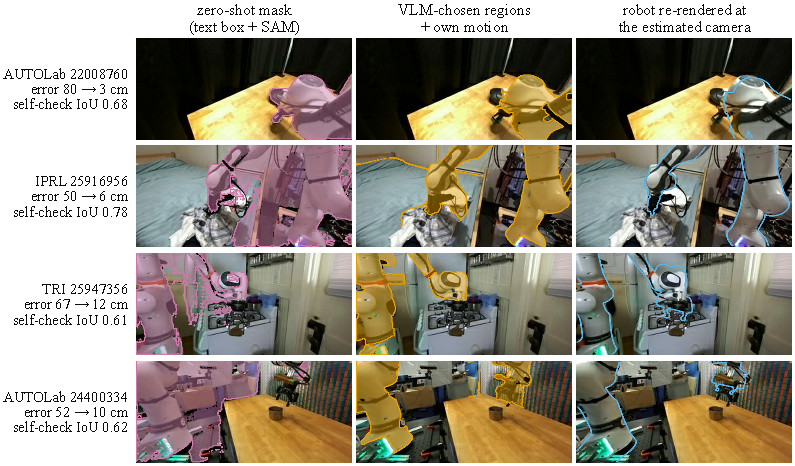
\includegraphics[width=\linewidth]{figs/droid_masks.pdf}
\caption{Real DROID frames, 4 of the 53 cameras (chosen to show one camera per failure mode of the zero-shot mask), with
the calibration error before and after and the ground-truth-free self-check IoU per row. Left: a zero-shot
text-box-plus-SAM mask (purple) attaches background to the robot. Middle: SAM regions chosen by a vision-language model
(orange), with part-robot regions split by the robot's own motion. Right: the robot re-rendered at the estimated camera
(blue outline). Over all 53 cameras, with identical search and only the mask changed, the median error is 25.4 cm /
$25.1^\circ$ zero-shot against 19.6 cm / $19.3^\circ$ VLM-chosen; under 30 cm 28 against 40, under 20 cm 19 against 28
of 53 (paired Wilcoxon $p=0.015$; the mask was changed after the registered stop rule had fired, so the change is post
hoc).}
\label{fig:droid}
\end{figure}
Offline calibration of DROID from robot masks is not new \citep{caliball,poseddroid}. What we add is why the obvious
pipeline fails and what repairs it: completing a mask with frame-to-frame motion re-attaches moving background unless
motion is trusted only inside regions already called robot (precision 0.91 falls to 0.75 otherwise), and keeping the
largest connected component drops parts of an arm cut by the frame edge (recall 0.68 to 0.53 on one camera). The
ground-truth-free self-check, the render IoU of the estimated camera, correlates with the true position error at
$\rho_s=-0.40$ ($p=0.003$, $n=53$)\ph; it was chosen after the data among three logged statistics (the calibration score
at the estimate, $+0.37$; the mask quality, $-0.14$). A dedicated robot segmenter \citep{robotseg} would be a natural
third mask source; the comparison here holds the search fixed and varies only the mask.

\paragraph{Why real-image calibration is harder.} On the 53 real DROID cameras, the true pose fits the observed masks
better than our estimate on only 18, which are search failures that a better optimiser could fix. On the other 35 the
loss itself prefers a wrong pose, because the real-image masks cover only part of the robot (median overlap with the
true silhouette 0.55, against 0.89 for our learned masks in simulation). Refinement cannot help those cameras, so on
real images the mask, not the optimiser, limits calibration.

\end{document}
